%!TEX root = ../thesis.tex
\chapter{Bayesian formalism}
\label{chap:BHM}
This chapter provides a general introduction to probability theory and its application to parametric inference. The objective of this work is to infer the probability distributions of the cluster properties (e.g. luminosity and velocity). Bayes' theorem provides the proper probabilistic framework for the inference of the parameters governing these distributions. The Bayesian framework demands, though, the setting up of prior beliefs about the parameters values. Thus, later in this chapter, I  describe the reason why the Bayesian Hierarchical Models are the least subjective to establish priors. Once the posterior distribution of the parameters in the model has been analytically described, I proceed to describe the MCMC techniques and the particular one I use to sample the posterior distribution. 

In the Sections ahead I also provide the details on the assumptions I make to model the data, and to choose the parameters of the prior distributions. The two final sections focus on the practical issues related to the sampling of the posterior distributions, and the description of the codes I adopted and/or developed.

\textbf{Partial results of the work presented here have been submitted to the journal A\&A as \citet{Olivares2017}. In the following, I use both pronouns \emph{we} and \emph{I} to refer the investigation done by collaborators of the DANCe team (see Chapter 1)}.

\section{Introduction to probability theory.}
\label{sect:introprobability}
 
Uncertainty and probability are closely entangled. Every measurement has an associated uncertainty, otherwise is not a complete measurement \footnote{Upper and lower limits are examples of incomplete measurements.}. The term uncertainty must not be confused with the term error, which refers to the difference between the measured value of the quantity and its \emph{true} value\footnote{The true value is that which ideally results when the uncertainty tends to zero.} \citep{GUM2008}. It is commonly agreed that the uncertainty of a measurement can be expressed in a probabilistic basis \citep{GUM2008}. It means that whenever we measure a quantity, $a$ for example, then the distribution of the repeated measurements of $a$, follows a probability distribution function, $p(a)$. Formally, if $a$ is a discrete variable, then its probability distribution is called probability mass function (PMF). On the other hand, if $a$ is continuous, then its probability distribution  is called probability density function (PDF). Throughout the text, I refer to the probability distribution function of a random variable as its probability distribution or simply its distribution.

Any probability distribution satisfies the following properties:

\begin{enumerate}[label=\textbf{Property \arabic*}]
\item  It has units, those of the inverse of $a$. \label{property:1}
\item $p(a) \geq 0 \ \ \forall \ \ a\in S_a$, with $S_a$ the support of $a$. \label{property:3}
\item $1=\int_{S_a} p(a) \mathrm{d}a$. \label{property:3}
\end{enumerate}

If $a$ is a discrete variable, then the integral, in the last property, change to the sum of all possible values of $p(a)$.

These properties hold regardless of the dimension of $a$. Furthermore, they also hold for conditional probability distributions. A conditional probability distribution results from the knowledge about the particular value of one or several variables of the probability distribution. For example, be $p(\alpha,\delta,\tau)$ the joint probability distribution of sky positions $\alpha,\delta$ and time $\tau$ of an object. Then, at the particular moment $\tau=\tau_0$ (with $\tau_0 \in S_{\tau}$) the object will have a probability distribution for its sky positions given by the conditional probability distribution $p(\alpha,\delta|\tau_0)$. Since, $p(\alpha,\delta|\tau_0)$ is still a probability distribution on $\alpha$ and $\delta$, it must also satisfy:

\begin{itemize}
\item It has units of $\alpha^{-1} \delta^{-1}$.
\item $p(\alpha,\delta|\tau_0)\geq0 \ \ \forall \ \ \alpha\in S_{\alpha}, \delta\in S_{\delta}$. %with $S_{\alpha}$ and $S_{\delta}$ the supports of $\alpha$ and $\delta$, respectively.
\item $1=\int_{S_{\alpha}} \int_{S_{\delta}} p(\alpha,\delta|\tau_0)\mathrm{d}\alpha\cdot \mathrm{d}\delta$.
\end{itemize}

The link between joint and conditioned probabilities is given by the following symmetric definition:

\begin{align}
p(a,b)=p(a|b)\cdot p(b).\nonumber \\
p(a,b)=p(b|a) \cdot p(a),
\end{align}

which can be further conditioned on $c$ to obtain:
\begin{align}
\label{eq:conditioned}
p(a,b|c)=p(a|b,c)\cdot p(b|c),\nonumber \\
p(a,b|c)=p(b|a,c) \cdot p(a|c).
\end{align}

If the joint probability of $a$ and $b$ can be factorised, this is
\begin{align}
p(a,b)=p(a)\cdot p(b),
\end{align}
then $a$ and $b$ are say to be \emph{independent}. An alternative option is to say that $a$ and $b$ are \emph{independent} if the conditional probability of $a$ on $b$ is $p(a|b)=p(a)$.

\textbf{
\ref{property:3} establishes that the amount of probability density\footnote{Which could be infinite, like in Dirac's delta.} (or mass if $a$ is discrete) spread over the volume of the support, adds to one, thus keeping the integrals of PDFs bounded. Two important operations using these bounded integrals are the following.
}

\textbf{
The \emph{marginalisation} of \emph{nuisance} parameters. These are parameters that, although are necessary in the model, lack interest for the research. The classical example of a nuisance parameters is the standard deviation, $\sigma$, of a normal distribution when the interest lies solely in the mean, $\mu$. This nuisance parameter can be marginalised from the joint PDF of the parameters, $p(\mu,\sigma)$, in the following way,
}
\begin{align}
\label{eq:marginalisation}
p(\mu)=\int_0^{\infty} p(\mu,\sigma)\cdot \mathrm{d}\sigma.
\end{align}

The computing of \emph{expected values}. The expected value of $a$, $E(a)$, corresponds to the mean of $a$ once we have drawn many realisations from its probability distribution. To compute it, we add all the possible values of $a$ weighted by their probability. This is,

\begin{align}
\label{eq:expectation}
E(a)=\int_a a\cdot p(a)\cdot \mathrm{d}a.
\end{align}

Once again, these last two equations (\ref{eq:marginalisation} and \ref{eq:expectation}) hold if the distributions are conditioned on any other measurement.

It is important to recall that the term measurement, and its unavoidable uncertainty, refer not just to directly measured quantities, like the photons (counts) and pixels in a CCD, but also to indirect measurements. Stellar magnitudes and positions in the sky, for example, are indirect measurements derived from the direct measurement of photons, pixels and telescope arrangements. This generalisation also applies to the measurement of parameters in any physical or statistical model.% like the one I will describe in the following Sections.


This Section ends with a brief description of the procedure that is generally applied when we want to transform a probability distribution into another probability distribution, under a nonlinear transformation \cite[for more details see for example][pages 18 and 19]{Bishop2006}. 

Let  $f$ be a probability distribution on $x\subset\mathbb{R}$, with support on $a<x<b$, then

\begin{equation}
\int_a^b f(x) \mathrm{d}x = 1 \nonumber
\end{equation}

Let $y=g(x)$ be the nonlinear transformation, with $g$ a function of $x$ with inverse $g^{-1}$, continuous and with continuous derivative, so that $x=g^{-1}(y)$, with $y\subset \mathbb{R}$. Then, the following is true,

\begin{equation}
\label{eq:transformdistribution}
\int_a^b f(x) \mathrm{d}x = \int_{g(a)}^{g(b)} f(g^{-1}(y))\cdot \left|\frac{\mathrm{d}g^{-1}(y)}{\mathrm{d}y}\right|\cdot \mathrm{d}y.
\end{equation}

\subsection{Bayes theorem}
The definition of conditioned probability (Eq. \ref{eq:conditioned}) leads to Bayes' theorem:
\begin{equation}
p(a|b,c) = \frac{p(b|a,c)\cdot p(a|c)}{p(b|c)}.
\end{equation}
Integrating on $a$ we find that,
\begin{align}
\label{eq:evidence}
p(b|c) \cdot \int_a p(a|b,c)\cdot \mathrm{d}a = \int_a p(b|a,c) \cdot p(a|c) \cdot \mathrm{d}a \nonumber \\
p(b|c) = \int_a p(b|a,c) \cdot p(a|c) \cdot \mathrm{d}a.
\end{align}
This Equation illustrates that $p(b|c)$ is a normalisation constant which can be evaluated once $p(b|a,c)$ and $p(a|c)$ are known. This turns out to be very useful, since it tells us that $p(a|b,c) \propto p(b|a,c) \cdot p(a|c)$.

\subsubsection{Models and parametric inference}
\label{sect:parametric_inference}
In a broad sense, models are representations or abstractions of the knowledge someone has about something. Sometimes this knowledge is also shared by others. Models are everywhere in our daily life: from the words we speak every day, to the evolution of the species and the general relativity; from a kid's drawing to cosmological models. In science, however, the concept of model is restricted to a mathematical representation of the relations (the knowledge) among the entities that the model attempts to describe: the observables (i.e. the data). If the model contains variables that through the different values they take reproduce in some extent the observables, then model is called parametric and the variables the parameters. 

\textbf{Parametric statistical models, like the ones I use in this work, assume that the underlying population of interest, from which the observed data is just a sample, can be described by parametric probability distribution functions. The act of finding the parameters governing these distributions is called parametric inference. This last can focus either on the entire PDFs of the parameters, or just on some summary of them (e.g. the maximum a posteriori, also known as MAP, or the mean and variance).}

The proper way to obtain the entire probability distribution of the parameters in a model, given the data, is through Bayes' theorem. Thus it is called Bayesian inference. Another example of parametric inference is the maximum likelihood approach, where the likelihood, which is seen as a function of the parameters, is maximised. Despite that it obtains the parameter values that make the model to resemble the data, it does not return their probability distribution. Formally, the likelihood is a probability distribution for the data, and just a function of the parameters. Thus, to obtain the probability distribution of the parameters, the likelihood must be multiplied by the priors and the product normalised. This is what Bayes' theorem does.

In this context, Bayes' theorem is:
\begin{equation}
p(\boldsymbol{\theta}|\mathbf{D},\mathcal{M}) = \frac{p(\mathbf{D}|\boldsymbol{\theta},\mathcal{M})\cdot p(\boldsymbol{\theta}|\mathcal{M})}{p(\mathbf{D}|\mathcal{M})}.
\end{equation}
where $\boldsymbol{\theta},\mathbf{D}$ and $\mathcal{M}$ correspond, respectively, to the parameters in the model, the data which the model tries to describe, and the model itself. 

The term on the \textbf{left-hand side} is called the posterior probability distribution of the parameters, $\boldsymbol{\theta}$ given the data $\mathbf{D}$, and the model $\mathcal{M}$. On the right hand side, the two terms in the numerator are called the \emph{likelihood} for the data, $p(\mathbf{D}|\boldsymbol{\theta},\mathcal{M})$ and the \emph{prior} of the parameters, $p(\boldsymbol{\theta}|\mathcal{M})$. The denominator, $p(\mathbf{D}|\mathcal{M})$, is called the \emph{evidence}, and results from

\begin{equation}
\label{eq:evidence}
Z \equiv p(\mathbf{D}|\mathcal{M}) = \int_{\boldsymbol{\theta}} p(\mathbf{D}|\boldsymbol{\theta},\mathcal{M})\cdot p(\boldsymbol{\theta}|\mathcal{M})\cdot \mathrm{d}\boldsymbol{\theta}
\end{equation} 

Formally, the likelihood and the prior are probability distributions for the data $\mathbf{D}$ and of parameters $\boldsymbol{\theta}$, respectively. However, for the posterior to be a probability distribution of the parameters, it only suffices that the product of the likelihood times the prior does not vanish everywhere or be negative anywhere\footnote{See Property 2. Although negative probabilities may have sense in quantum mechanics. See for example \citet{1942RSPSA.180....1D}}. If these are not probability distributions, they are called \emph{improper} priors or \emph{improper} likelihoods. In the extreme case that their product vanishes everywhere, which may be the case if the prior is terribly specified or if the likelihood does not take proper account of extreme data, the posterior will not be a probability distribution due to a division by zero. Nevertheless, it makes no sense to try to estimate the parameters of a model with zero evidence.

%Whenever we have a model $M$, we have also the \emph{a priori} knowledge used to construct it. Actually, it can be classified in two kinds of prior information. One refers to the prior information conveyed in the model, which I call $M$. This is the information that the creator of the model uses to establish the relations among the elements of the model: variables. The second kind of prior, $p(\boldsymbol{\theta}|M)$ refers to the statement the user of the model made of his/her beliefs about the probability distribution of the parameter values. This is indeed subjective. However, it is, in my opinion, less subjective than the former, $M$, prior information. At least in this last kind, the subjectivity is expressed objectively in a probabilistic, and therefore measurable way.
%
%The likelihood of the data $p(\mathbf{D}|\boldsymbol{\theta},M)$, is a probability distribution on the data, $\mathbf{D}$. However, it is a function on the parameters, $\boldsymbol{\theta}$, which corresponds to the function $f$ of Eq. \ref{eq:model}. This function is not necessarily a probability distribution on the parameters. 

As mentioned before, the likelihood is a probability distribution for the data, given the parameters, regardless of the size of it. Almost always the data is a collection of measurements of several objects, but it could also be made up of just one object. The collection of measurements of one or several quantities of a single object follows a probability distribution, which is usually summarised by two statistics. It is often assumed that this probability distribution is normal (univariate or multivariate), which then is summarised by the mean and the standard deviation. These two are commonly known as the datum and its uncertainty, respectively. A data set is then composed of the collection of summary statistics of one or several objects. To compute the likelihood for this collection of statistics (i.e. the data), some assumption must be made. 

When measuring the properties of objects, it is often assumed that the probability distribution obtained from the collection of measurements of a single object, is independent from that of another object. For example, if we were to measure the weight of a group of persons, we usually assume that the PDF of the weight of one person, is independent of that of another person. It means that measuring the weight of one person has no effect at all in the weight of another person.


In this work it is always assumed that the PDFs of the measured quantities of individual objects are independent amongst them. Nevertheless, in the following, I give an example where this assumption may not be entirely right. Obtaining stellar positions in celestial coordinates often requires what is called an astrometric solution. This solution is a map from the raw data, like pixel positions in the detectors and observing epoch, to the celestial coordinates (e.g. right ascension, declination and epoch). This astrometric solution often needs large collections of measurements of the same objects, so that they can be robustly estimated. Since this mapping is computed from the data (e.g. using maximum-likelihood estimates) and then applied to the same data, then it is common to observe correlations among the uncertainties of different objects \cite[see for example][]{2010IAUS..261..320H,2017A&A...601A..19G}. If the correlation in the uncertainties is significative, then their PDFs are probably not independent\footnote{Independent PDFs produce uncorrelated samples, however, uncorrelated samples do not imply independence between the PDFs of their underlying populations.}.  


Let $\mathbf{D}$ be the data, i.e. the collection of statistics of the $N$ objects, and $p_n(\mathbf{d}_n)$ be the probability distribution rendered by several measurements of object $n$. If these $\{p_n(\mathbf{d}_n)\}_{n=1}^N$ are assumed to be independent, then
\begin{equation}
\label{eq:independence}
 p(\mathbf{D}) = \prod_{n=1}^N p_n(\mathbf{d}_n),
\end{equation}

 with $p_n$ explicitly stating that the individual probability distributions are distinct. 
 
Similarly, if the likelihood of the data, $p(\mathbf{D}|\boldsymbol{\theta},M)$ is assumed to be independent for each object, then

\begin{equation}
\label{eq:lik_datum}
 p(\mathbf{D}|\boldsymbol{\theta},M) = \prod_{n=1}^N p(\mathbf{d}_n|\boldsymbol{\theta},M).
\end{equation}

The term $p(\mathbf{d}_n|\boldsymbol{\theta},M)$ is the likelihood of datum $\mathbf{d}_n$. This is also called the \emph{generative} model, since it contains the necessary information to generate the data. 


To take into account the uncertainty process for object $n$, we model the datum $\mathbf{d}_n$ as resulting from the addition of the true value, $\mathbf{x}_n$, which is given by the model, with a random variable, $\mathbf{e}_n$, given by the uncertainty process. This is
\begin{equation}
\mathbf{d}_n = \mathbf{x}_n + \mathbf{e}_n. \nonumber
\end{equation}

In general, if the model does not contain any intrinsic dispersion, then its likelihood can be thought of as a Dirac $\delta$ function, which is centred at the \emph{true} value $\mathbf{x}_n$. Then, it can be added (i.e. convolved\footnote{The addition of two random variables results in another random variable. This is analogous  to the convolution, dennoted $*$, of their PDFs.}) to the distribution of the uncertainty process. However, it is customary to also include an intrinsic dispersion in the model to account for over-simplistic assumptions or underestimated uncertainties. 

In particular, it can be assumed that both the uncertainty process of datum $\mathbf{d}_n$, and the likelihood of the model are normally distributed with variances $\boldsymbol{\Sigma}_n^2$ and $\boldsymbol{\Sigma}^2$, respectively, 
\begin{align}
p(\mathbf{e}_n|\mathbf{\Sigma}_n^2)= &\mathcal{N}(\mathbf{e}_n|0,\boldsymbol{\Sigma}_n^2), \nonumber\\
p(x_n|\boldsymbol{\theta},M,\mathbf{\Sigma}^2)= &\mathcal{N}(\mathbf{x}_n|\boldsymbol{\theta},M,\boldsymbol{\Sigma}^2).\nonumber
\end{align}
Formally, $\boldsymbol{\Sigma}^2$ is part of the set of model parameters, $\boldsymbol{\theta}$, but I explicitly leave it outside to exemplify the process. 

Then the addition of these two normally distributed random variables results in another normally distributed random variable\footnote{The convolution of two Gaussian PDFs is another Gaussian PDF.}. Thus,

\begin{equation}
p(\mathbf{x}_n|\boldsymbol{\theta},M,\boldsymbol{\Sigma}^2)*p(\mathbf{e}_n|\boldsymbol{\Sigma}_n^2) = \mathcal{N}(\mathbf{d}_n|\boldsymbol{\theta},M,\boldsymbol{\Sigma}_n^2+\boldsymbol{\Sigma}^2).
\end{equation}

Therefore, Eq. \ref{eq:lik_datum}, can be expressed in general as,

\begin{equation}
\label{eq:lik_generativemodel}
p(\mathbf{D}|\boldsymbol{\theta},M) = \prod_{n=1}^N p(\mathbf{d}_n|\boldsymbol{\theta},M,\mathbf{u}_n),
\end{equation}
where $\mathbf{u}_n$ is the uncertainty of datum $\mathbf{d}_n$.


Bayes' theorem can be interpreted as the probabilistic way to update the state of knowledge. To me, it embodies the process of knowledge improvement once we recognise that knowledge is uncertain. Even when its uncertainty is negligible under the evidence that supports it. Bayes' theorem helps us update our prior beliefs once we multiply it by the likelihood of the data. Then, the posterior probabilities, become our new state of knowledge. 

Furthermore, Bayes' theorem also provides the objective way to compare two models or hypothesis, and update the a priori knowledge used to construct them. This is called model selection, which I  briefly explain in the next section.

\subsection{Model Selection}
\label{sect:modelselection}

Whenever we have a data set and two or more models that attempt to describe these data, the most straightforward thing to do is to compare these models. Almost always, we want to select the \emph{best} model. Obviously the term \emph{best} depends on the objective of the research. For example, imagine that our data set consists of the positions of an object as function of time. If we were interested in reproducing exactly the same points in the data set, the \emph{best} model would be a polynomial with degree equal to the number of points. This polynomial will pass through all the points. However, once we recognise the unavoidable uncertainty of the data, we realise that an exact representation of the data may be of no use since it fits also the noise. 

In general, we are interested in the predictive capabilities of a model, its ability to predict future observations rather than to replicate the ones we currently have. Thus, an exact representation of the observed data (an over-fitted model as in the previous example), will poorly describe any new data. In this sense, an over-fitted model \emph{memorises} the data rather than \emph{learns} from it.

A model that \emph{learns} from the data is that which recovers the \emph{true} underlying relation embedded in the data. This \emph{true} underlying relation is the one that produces the \emph{true} data. The observed data results once the uncertainty is added. 

Nevertheless, we still need to select among different learning models.  

We can draw some help from the commonly known Ockham's razor or principle \footnote{The origin of this motto and its exact phrasing is beyond the scope of this work. I just mention that paradoxically, an ancient formulation is attributed to Ptolomey: "We consider it a good principle to explain the phenomena by the simplest hypothesis possible" \citep{Franklin2002}}. It says:
\begin{quotation}
\textit{Among competing hypotheses, the one with the fewest assumptions should be selected.}
\end{quotation}

Here, hypotheses can be identified with models. Thus, this principle tells us we should choose the model that makes the fewest assumptions. I classify the assumptions of a model in two groups: fixed and free ones. The fixed assumptions belong to what I previously described as the \emph{a priori} knowledge used to construct the model. These may render the model more interpretable in the physical or statistical sense, or even give it coherence within the corpus of a theory. The free assumptions on the other hand, correspond directly to the parameters in the model. They give it flexibility when fitting the data\footnote{However, they can also introduce degeneracy in the parametric space.}. For example, in the case of a straight line model, the fact that the data is linearly related can be considered as a fixed assumption. The free assumptions correspond to the slope and ordinate at the origin. 

When comparing a linear model to a quadratic one in which the constant term has been fixed, we see that they have the same number of free parameters, two, but clearly the second one has an extra fixed assumption. Therefore, choosing the model with fewer free parameters does not necessarily means choosing the model with the fewest assumptions.

One of the great advantages of the Bayesian methodology is that it incorporates directly Ockham's principle. Suppose that we want to compare two models, $M_1$ and $M_2$, which we assume describe the data set, $\mathbf{D}$. Each model has prior probabilities, $p(M_k)$ and likelihoods $p(\mathbf{D}|M_k)$ (with $k=1,2$). Notice that now, I use Bayes' theorem for models and not for parameters within a model. So, the prior probabilities of the models reflect our beliefs about the fixed assumptions within each model. On the other hand, the likelihood of the data, given the model, is related to the parameters (the free assumptions) and their prior probabilities, both within a model. This likelihood of the data given the model corresponds to the \emph{evidence} of the model (Eq. \ref{eq:evidence}). This evidence, written in terms of the model parameters, $\theta_k$, is now

 \begin{equation}
p(\mathbf{D}|M_k)=\int_{\theta_k} p(\mathbf{D}|\theta_k,M_K)\cdot p(\theta_k|M_k)\cdot \mathrm{d}\theta_k. \label{eq:evidence2}
\end{equation}
Bayes' theorem applied to models, instead of individual parameters as illustrated above, tells us that
\begin{equation}
p(M_k|\mathbf{D})=\frac{p(\mathbf{D}|M_k)\cdot p(M_k)}{p(\mathbf{D})},
\end{equation}
with $k=1,2$. Since there are only two models, their prior probabilities are related by $p(M_1)= 1- p(M_2)$. Therefore,
 \begin{equation}
p(M_k|\mathbf{D})=\frac{p(\mathbf{D}|M_k)\cdot p(M_k)}{p(\mathbf{D}|M_1)\cdot p(M_1)+p(\mathbf{D}|M_2)\cdot p(M_2)}.
\end{equation}
From this last Equation, the ratio of the posterior distributions is:
\begin{equation}
\frac{p(M_1|\mathbf{D})}{p(M_2|\mathbf{D})}=\frac{p(\mathbf{D}|M_1)\cdot p(M_1)}{p(\mathbf{D}|M_2)\cdot p(M_2)}.
\end{equation}
This ratio provides an objective measure of how better the model $M_1$ is when compared to model $M_2$, under the measure provided by the data $\mathbf{D}$ by means of the evidence. When both prior probabilities  $p(M_1)$ and $p(M_2)$ are set alike, the ratio of posteriors equals the ratio of likelihoods. This is known as the \emph{Bayes factor} \cite[for a similar derivation and some examples of its application see][]{Kaas1995}. 

Even when the priors for the models are set alike, the evidences themselves (Eq. \ref{eq:evidence2}) embody Ockham's principle. The evidence is the integral, in parametric space, of the prior times the likelihood, with the likelihood acting as a weight to the priors.  Then, the larger the number of parameters (free assumptions) is, the greater the volume over which the integral must be carried on, and the most spread the prior probability gets. Thus, unless the likelihood increases as well, the evidence is smaller in models with larger number of parameters.

As explained in this section, the paramount importance of Bayes' theorem comes from the fact that it is the proper probabilistic way to update knowledge based on the \textbf{statistical} evidence.

\subsection{Membership probability}

In the previous Section we \textbf{derived} the ratio of the probabilities of two competing models $M_1$ and $M_2$, given the data $\mathbf{D}$. In this Section, I describe a similar problem: the probability of two competing models given the two likelihoods for a single datum, $\mathbf{d}$. It also can be interpreted as the probability that the datum $\mathbf{d}$ was generated by model $M_k$. This probability is commonly known as the membership probability of the datum $\mathbf{d}$ to belong to model or class, $M_k$ ($k=1,2$). 

Bayes' theorem for this particular case is,

\begin{equation}
\label{eq:prob}
p( M_k | \mathbf{d}) =\frac{p(\mathbf{d}|M_k)\cdot p(M_k)}{\sum_{k=1}^2 p(\mathbf{d}|M_k)\cdot p(M_k)},
\end{equation}

where $p(\mathbf{d}|M_k)$ is the likelihood of datum $\mathbf{d}$ and, $p(M_k)$ is the prior probability of model $M_k$.



\section{Bayesian Hierarchical Models}
\label{sect:BHM}
\subsection{Generalities}
\label{sect:generalities}
The Bayesian formalism requires the establishment of priors. These represent the beliefs the user of the model has about the possible values that parameters of the model can take \textbf{before new data are observed}. This is indeed subjective. This subjectivity is the main source of criticism from the non-Bayesian community \footnote{See \citet{Gelman2012} for a discussion on the ethical use of prior information}. 

Bayesian hierarchical models, in the following BHM, are classified within the Empirical Bayes methods. On these methods, the prior distributions are inferred from the data rather than being directly specified, as it is done in common Bayesian methods. In BHM the priors are specified by parametric distributions whose parameters are also drawn from another parametric distribution in a hierarchical fashion. For this reason, hierarchical models are also called multilevel models. A full-BHM is that in which the parameters at the higher hierarchy \textbf{level} are drawn from a non-parametric distribution. In a non full-BHM the settlement of parameters stops at some level. These end-level parameters are called hyper-parameters.

Given their properties, BHMs represent the most objective way to the establishment of prior distributions \citep{Gelman2006}. Regardless of the level of the BHM, for it to be effective, the family, or class, of prior distributions must be carefully chosen. These families must allow the \emph{true} value of the parameter of interest \citep{Morris1983}. If the likelihood \textbf{parametric support} is not fully contained in the prior (for example when the likelihood, as a function of the parameters, has a maximum outside the domain of a truncated prior), then the inferred posterior \textbf{can} be biased. For this reason, inspecting the prior knowledge is an important step in any Bayesian study.

Despite their theoretical advantages, BHMs are difficult to evaluate since they require far more parameters than standard Bayesian methods.
Furthermore, their hierarchy (levels) must stop at some point. There are at least two approaches to stop this hierarchy. The first one uses a non-parametric distribution for the parameters at the higher level. This renders, as previously noted, a full-BHM. \textbf{However, it demands an a priori knowledge of the non-parametric distribution, which, most of the time, is not the case.} The second option is to give a point estimate, usually the mean or the mode, for the distribution of the parameter at the top of the hierarchy.  


Although in BHMs the parameters of the prior distributions are inferred from data, the user of the model has the important task of specifying the family of distributions to be used for them. Selecting these families continues to be an active area of research. The most common approaches are the following.

\begin{itemize}
\item Conjugate priors. In this kind of priors the posterior distribution, which results of the product of the prior times the likelihood, is also in the same family distribution of the prior. 

\item Default priors. These priors are used when there is insufficient information to set the prior and are supposed to be the default choice in the absence of any other information. 

\item Reference priors. Formally, a reference prior is permissible and maximise the missing information. See \citet{Berger2009} and references therein.

\item Non-informative priors. This kind of priors intentionally discards all information on the phenomenon.

\item Weakly informative priors. These provide intentionally weaker information than what actually is. 
\end{itemize}

The default and non-informative approaches are discarded since for the Pleiades, which is one of the most studied cluster in the literature, there is already reliable information which must be used.  Conjugate priors do not always agree with the previous knowledge. Reference priors, although an interesting approach, require complicated derivations which are hard to implement and thus computationally expensive. 

From the previous options, I choose the weakly-informative approach. These are recommended by \citet{Gelman2006,Gelman2008,Huang2013} and \citet{Chung2015}, since they show better computational performance when compared to non-informative priors.

Whatever family used for the prior distribution, we must always analyse the priors in terms of the posterior distribution, and check if the late makes sense \cite[][ Chap. 6]{Gelman2006,Gelman2013}.


\subsection{Examples}
Since BHMs usually need more parameters than standard techniques, its use was restricted until fast computers were widely available. The concept of BHM was already present in the 1960s. However, it was not until  the 1970s that they were used to infer parameters of normal distributions and linear models \cite[see][for an historical perspective of BHMs]{Good1980}. In modern days, BHMs have a wide range of applications. Just to cite some examples, \citet{Gelman2007} use them in the social sciences, \citet{Fei2005} applies them for vision recognition and, \citet{Diard2008} for robot navigation.

BHMs are also widely applied in astrophysics. Although, originally its use was mainly in the domain of inference of cosmological parameters \cite[see for example the works of][]{Feeney2013,March2014,Anderes2015,Shariff2016,Alsing2017}, they were rapidly adopted in other domains. For example, they have been used to study the eccentricity distribution of binary stars \citet{Hogg2010}, the Cepheids \citep{Barnes2004} and RR Lyrae distances \citep{Jefferys2007}, the chemical composition \citep{Wolfgang2015} and albedos of exoplanets \citep{Demory2014}, extinction maps \citep{Sale2012}, stellar parameters \citep{Shkedy2007}, and the present day mass distribution \citep{Tapiador2017}.

\subsection{Graphical representation.}
\label{sect:PGM}
Probabilistic Graphical Models (PGM) provide the background to graphically depict BHMs. PGMs are graphs that portray the conditional relations among the elements in a probabilistic model. These elements can be constants or stochastic variables that interact by means of conditional relations, which can in turn be deterministic or stochastic. 

In PGMs, stochastic variables are represented with circles and constants with squares. If the variable is known, as in the case of the data, it is represented with a filled symbol, otherwise with an empty symbol. Stochastic and deterministic relations are depicted with solid and dashed lines, respectively. If there is no line between two given elements, it indicates that they are assumed to be independent. Variables that repeat together, as in the case of the data, are grouped within a plate. The number of repetitions is indicated in one corner of the plate. For more details on PGMs see for example the book of \citet{Koller2009}. 

To exemplify the use of PGMs, Figure \ref{fig:pgmGMM} shows the PGM for the BHM that infers the parameters in a Gaussian Mixture Model. In this model the parameters are the means $\mu_k$, variances $\sigma_k^2$ and fractions $\phi_k$ of each of the $K$ gaussian distributions in the mixture. Then $\mu_0,\sigma_0^2,\lambda,\nu$ and $\beta$ are the hyper-parameters, while $x_i$ represent the data, and $z_i$ the categorical latent variable that indicates the parent gaussian for datum $x_i$. The squiggly line ending in T indicates that $z_i$ is switch, which selects the gaussian at which $x_i$ belongs.

\begin{figure}[ht!]
\begin{center}
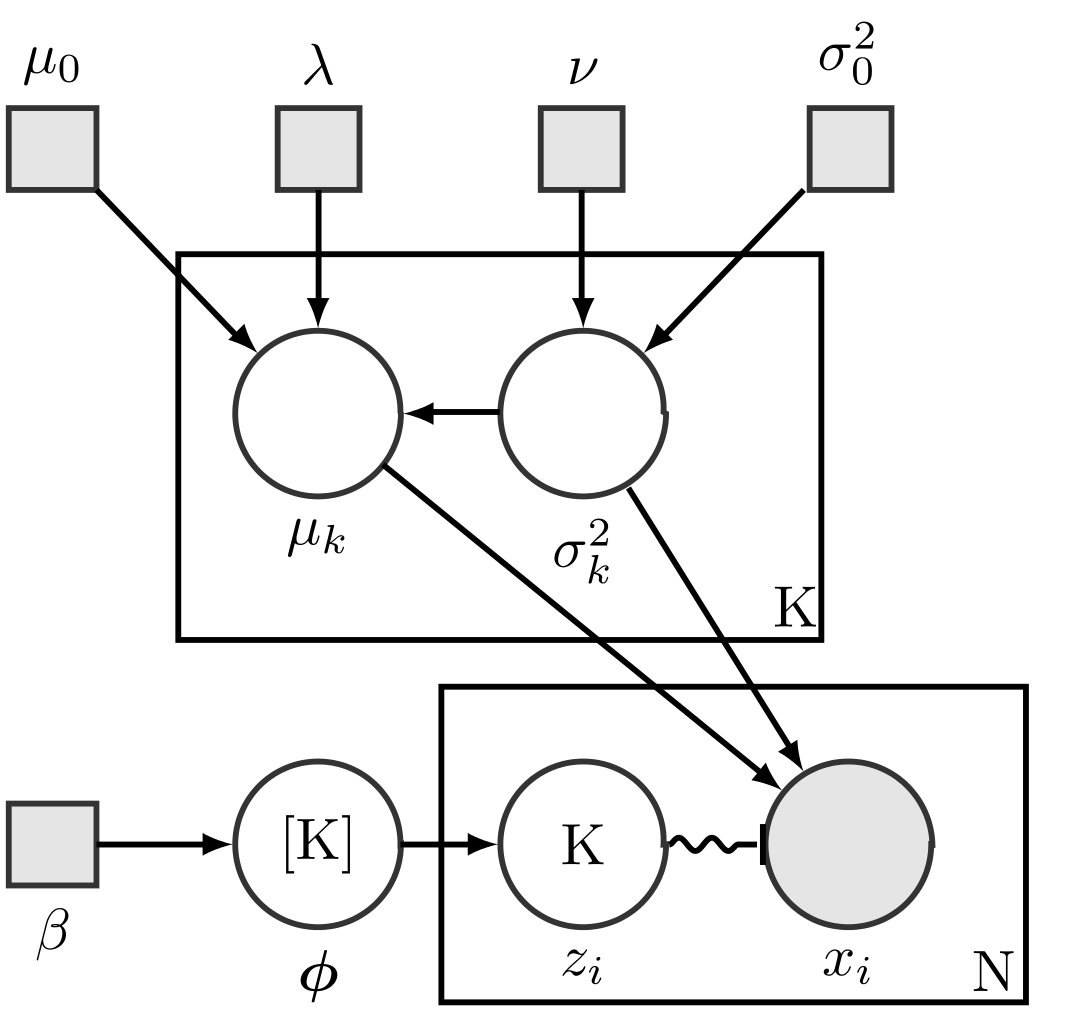
\includegraphics[height=8cm]{background/Figures/BGMM.png}
\caption{PGM representing the parametric inference of a Gaussian Mixture, see text for details. Figure by Benwing, license: Creative Commons BY-3.0}
\label{fig:pgmGMM}
\end{center}
\end{figure}

\section{The BHM for the Pleiades DANCe data set}
\label{sect:datamodelling}
Creating a model is a complex task. As previously mentioned, a model is a mathematical representation of the knowledge about a certain phenomenon. Thus, a model demands the gathering and arranging of the \emph{a priori} knowledge of the phenomenon as well as the gathering process of its associated data set. 

The current understanding of the Pleiades cluster together with the description of the DANCe DR2 data set are summarised in Chapter \ref{chap:pleiades}. 

Once the \emph{a priori} knowledge has bee gathered, the creation of the model becomes an iterative and continuous process. Assembling the knowledge into a coherent system demands continuous iterations of decision making, test, and analysis of preliminary results. This Section provides a snapshot of this process: the state of the model once the article \citet{Olivares2017} was submitted.

Section \ref{sect:missing} explains the statistical procedure to deal with one of the crucial aspects of the Pleiades DANCe DR2 data set: objects with missing values in their measurement vector. Later, Section \ref{sect:generative-model} provides details of how the relevant knowledge about the Pleiades cluster and field populations are embedded in the generative model of the data.
\subsection{Missing values}
\label{sect:missing}

Missing values refer to a non-measured or non-available (NA) value in the vector of measurements of an object. They can arise due to different statistical or physical processes. 

From the physical perspective, they occur due to faint or bright sources that produce counts values outside the dynamical range of the detector. They can also emerge due to detector malfunctions, e.g. electronic failures, or to random effects, e.g. cosmic rays. 

From the statistical perspective, important aspects of missing values are, i) the probability distribution of the sources in which they occur, and ii) if they originate due to censoring or truncation. 

In the DANCe DR2, missing values occur only in the photometric measurements (see Table \ref{tab:DR2properties}), with the bluer bands being the most affected. As expected, the probability distribution of sources with missing values is not \textbf{uniform}. Missing values occur with higher probability at the faintest and brightest ends of the photometric distributions, see Figure \ref{fig:NAsKs}. This is a crucial aspect for the statistical analysis. If missing values were \textbf{uniformly} distributed, then, any statistical analysis derived using only objects with completely observed vectors would be unbiased. This will occur because the objects with completely observed vectors would be a random sample of the data set. \textbf{Since this is not the case in the DANCe DR2, objects with missing values must be incorporated in the data set and properly treated to avoid biases.} 

\begin{figure}[ht!]
    \centering
    \begin{subfigure}[t]{0.45\textwidth}
        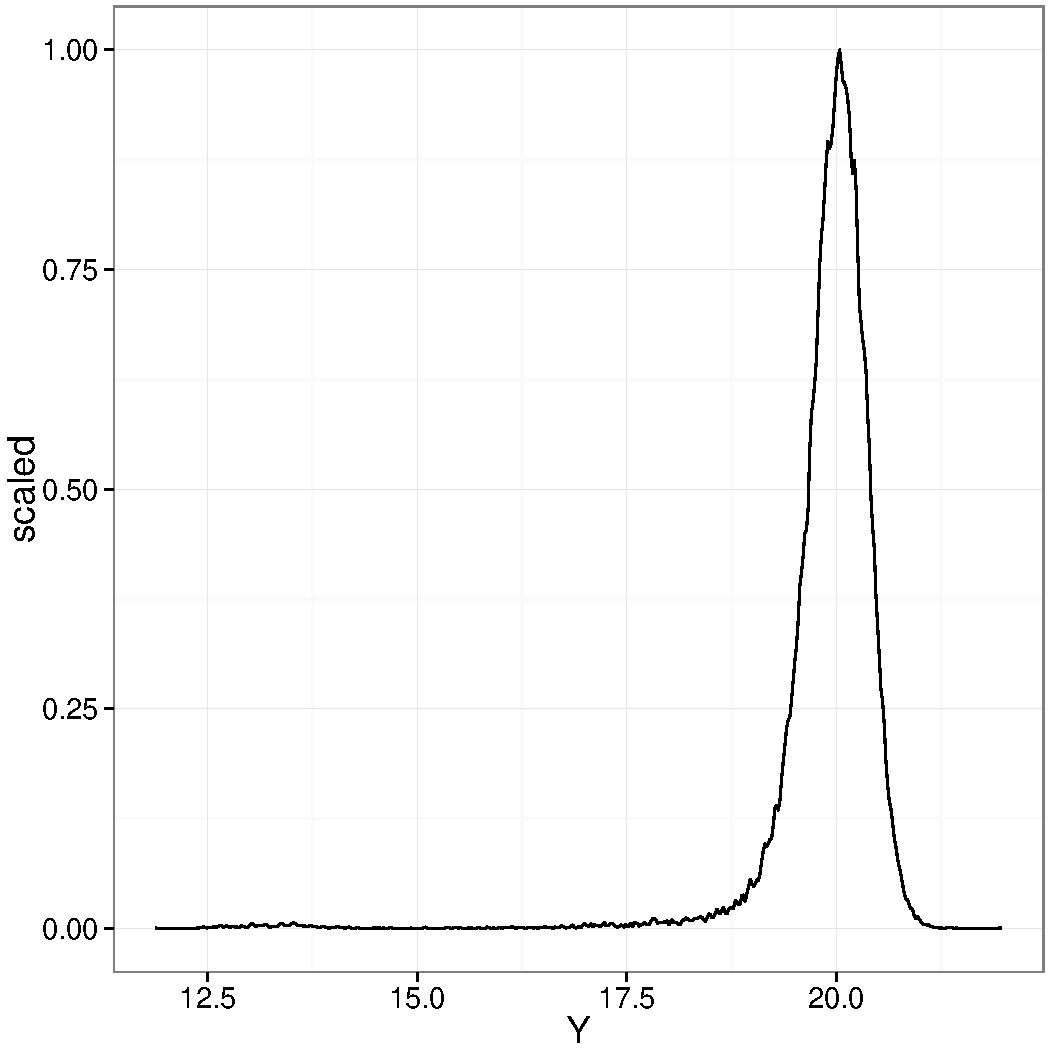
\includegraphics[page=1,height=6cm]{background/Figures/MissingDistribution.pdf}
        \caption{}
        \label{}
    \end{subfigure}
    \begin{subfigure}[t]{0.45\textwidth}
      \includegraphics[page=2,height=6cm]{background/Figures/MissingDistribution.pdf}
        \caption{}
        \label{} 
    \end{subfigure}
     \begin{subfigure}[t]{0.45\textwidth}
      \includegraphics[page=3,height=6cm]{background/Figures/MissingDistribution.pdf}
        \caption{}
        \label{} 
    \end{subfigure}
     \begin{subfigure}[t]{0.45\textwidth}
      \includegraphics[page=4,height=6cm]{background/Figures/MissingDistribution.pdf}
        \caption{}
        \label{} 
    \end{subfigure}
\caption{Probability distributions of objects with missing values. The vast majority of objects with missing values are located at the faint end of the magnitude distributions.}
\label{fig:NAsKs}
\end{figure}




\textbf{Truncation occurs when the data set does not contain records, neither of the measured value nor of the number of measurements, for objects whose measured quantity lies outside certain limits}. On the other hand, censoring happens when the data set contains only partial information about the actual value of the measured quantity. Basically,  censoring happens when the value lies outside the upper or lower limits of the measuring instrument, and these limits become the only available record of the measurement. Currently, the DANCe DR2 does not provide upper or lower limits for the censored data. Although these limits could also be inferred from the data, the heterogeneous origin of the DANCe DR2 prohibits this task. Furthermore, the missing values in the DANCe DR2 data set do not occur only because of censoring. Indeed, cosmic rays, hot pixels, halos of bright stars, diffraction patterns and cross-matching failures are just some examples of potential sources of missing values. The statistical treatment of missing values originating from all these sources lies beyond the scope of this work. However, there is a general way to deal with missing values \textbf{whatever} their origin.

In terms of probability, there is no distinction between missing values and parameters. Therefore, we can marginalise missing values as we do with any other nuisance parameter. If the vector of measurements $\mathbf{d}$ has a missing value in entry $i$, then $x_{i} = NA$ , and $\mathbf{d}=\{x_1,x_2,...,x_{i-1},NA,x_{i+1}...,x_n\}$, with $n$ the dimension of $\mathbf{d}$. Thus, the marginalised likelihood of this datum, given model parameters $\boldsymbol{\theta}$ is

\begin{equation}
\label{eq:marginalmiss}
p(\mathbf{d}|\boldsymbol{\theta})= \int_{-\infty}^{\infty} p(\{x_1,x_2,...,x_{i-1},x_{i}= NA,x_{i+1},...,d_n\}|\boldsymbol{\theta})\cdot \mathrm{d}x_{i}.
\end{equation}

Throughout this work, missing entries are marginalised in the previous way whenever present.

%I made a remark of a point that may seem obvious but it is important to remember. Let $p(a)$ be a probability distribution, $A$ a random sample of $n$ points from it, and $p_A(a)$ the empirical probability distribution of $A$. Let $B$ be a non-random sample of $p(a)$ with $n$ elements, and empirical probability distribution $p_B(a)$. In the limit of $n\rightarrow \infty$, $p_A(a)=p(a)$ however $p_B(a)\neq p(a)$. Therefore, $p_A(a)\neq p_B(a)$. Similarly, in data with missing values, if the missing value pattern is not random, the distribution of the completely observed data (with non-missing values) differs from that of all the data. In \citet{Olivares2017} we show this subtle but important difference in the case of the DANCe data set. 

\subsection{The generative model}
\label{sect:generative-model}
\textbf{In the Pleiades DANCe DR2 data set, cluster stars are mixed with field sources. Thus, cluster and field populations must be disentangled to achieve the objective of this work. The probabilistic disentanglement of them, requires probabilistic models for each population, i.e. their likelihoods. The true values of these two likelihoods, field and cluster, are given by parametric relations embodying the state of knowledge of NYC.  Using these likelihoods, individual cluster membership probability PDFs are computed (by means of Eq. \ref{eq:prob}) for each object in the data set. These PDFs together with a probability classification threshold,  allow individual objects to be separated into cluster and field populations.}

The inference process demands a set of $N$ binary integers $\mathbf{q}$, one $q_n$ for each object. The two possible values of these binary integers represent one of the two mutually exclusive possibilities: the object belongs to the cluster ($q_n=1$) or to the field population ($q_n=0$). 

Let $\boldsymbol{\theta}$ and $\boldsymbol{\phi}$ be the parameters of the cluster and field models, and $p_c$ and $p_f$ their likelihoods, respectively. Then, the likelihood of the data, $\mathbf{D}$, is,

\begin{equation}
p(\mathbf{D}|\mathbf{q},\boldsymbol{\theta},\boldsymbol{\phi})= \prod_{n=1}^N {p_c(\mathbf{d}_n|\boldsymbol{\theta})}^{q_n}\cdot {p_f(\mathbf{d}_n|\boldsymbol{\phi})}^{(1-q_n)}.
\end{equation}

The inference of these $N$ binary integers will demand a computing power that is outside the current possibilities. Thus, instead of inferring them, I marginalise them using a prior probability, which is set in terms of a new and unique parameter $\boldsymbol{\pi}$. It represents the \emph{prior} probability that an object belongs to the field. Thus, the prior probability of $\mathbf{q}$ is

\begin{equation}
p(\mathbf{q}|\pi)= \prod_{n=1}^N {(1-\pi)}^{q_n}\cdot {\pi}^{(1-q_n)}.
\end{equation}

Since $\mathbf{q}$ represents the $2^N$ possible ways to combine the binary variables $q_n$, then the marginalisation over all these possible states is,

\begin{align}
p(\mathbf{D}|\pi,\theta,\phi)&=\sum_{\mathbf{q}} p(\mathbf{D},\mathbf{q}|\pi,\theta,\phi)\cdot \mathrm{\Delta}\mathbf{q} \nonumber\\
&=\sum_{\mathbf{q}} p(\mathbf{D}|\mathbf{q},\pi,\theta,\phi)\cdot p(\mathbf{q}|\pi)\cdot \mathrm{\Delta}\mathbf{q} \nonumber \\
&=\sum_{\mathbf{q}} \prod_{n=1}^N {p_c(\mathbf{d}_n|\theta)}^{q_n}\cdot {p_f(\mathbf{d}_n|\phi)}^{(1-q_n)}\cdot \prod_{n=1}^N {(1-\pi)}^{q_n}\cdot {\pi}^{(1-q_n)}\cdot \mathrm{\Delta}\mathbf{q} \nonumber \\
&=\sum_{\mathbf{q}} \prod_{n=1}^N \left[(1-\pi)\cdot p_c(\mathbf{d}_n|\theta)\right]^{q_n}\cdot \left[\pi\cdot p_f(\mathbf{d}_n|\phi)\right]^{(1-q_n)}\cdot \mathrm{\Delta}\mathbf{q} \nonumber \\
&=\prod_{n=1}^N (1-\pi)\cdot p_c(\mathbf{d}_n|\theta) + \pi\cdot p_f(\mathbf{d}_n|\phi).
\end{align}
This last equality is a rather complicated derivation which can be found in \citet{Press1997}, and in \citet{Hogg2010a} for $p_c$ and $p_f$ in the exponential family. Also, a general derivation of this expression is given by \citet{Jaynes2003}. He obtains it assuming individual unknown probabilities $p_n$ instead of $q_n$ and marginalising over them with the aid of a prior.

Thus, the \emph{generative model} or likelihood of the datum $\mathbf{d_n}$  is

\begin{equation}
\label{eq:genmod}
p(\mathbf{d}_n | \pi,\boldsymbol{\theta}_c,\boldsymbol{\theta}_f,\mathbf{u}_n)=\pi \cdot p_f(\mathbf{d}_n|\boldsymbol{\theta}_f,\mathbf{u}_n) + (1-\pi)\cdot p_c(\mathbf{d}_n| \boldsymbol{\theta}_c,\mathbf{u}_n),
\end{equation}

where $\boldsymbol{\theta}_f$ and $\boldsymbol{\theta}_c$ indicate the cluster and field parameters, while $\mathbf{u}_n$ refers to the datum uncertainty. The probabilities $p_f(\mathbf{d}_n|\boldsymbol{\theta}_f,\mathbf{u}_n)$ and $p_c(\mathbf{d}_n| \boldsymbol{\theta}_c,\mathbf{u}_n)$ are the field and cluster models, respectively. These models are explained in detail in the next two sections.

In the following, I assume that the observed quantities, even if they contain missing values, resulted from the convolution of likelihood, given the \emph{true} quantities, with the uncertainty process (see Section \ref{sect:parametric_inference}). The latter could be different for each object, thus resulting in different individual uncertainties. It means that the DANCe DR2 data set is modelled allowing for its intrinsic heteroscedaticity. Although these uncertainties are not assumed to have the same values, I do assume that they have the same shape. Thus, I assume that uncertainties in our data set belong to the multivariate normal family.  This assumption is standard practice and is also supported by the large and heterogeneous origins of the DANCe DR2 data set. 

\subsection{The field population}
To model the field population, I assume that the joint seven-dimensional probability distribution of the field can be factorised into the probability distributions of proper motions and photometry. Thus, the field likelihood of the proper motions and the photometry are assumed to be independent. Also, I assume that both distributions are described by Gaussian Mixture Models (GMM). The flexibility of GMMs to fit a variety of distribution geometries makes them a suitable model to describe the field density of the heterogeneous DANCe DR2 data set. 

\textbf{A GMM is a probability distribution resulting from the linear combination of $M$ Gaussian distributions, }
\begin{equation}
p_{GMM}(x|\boldsymbol{\pi},\boldsymbol{\mu},\boldsymbol{\Sigma})=\sum_{m=1}^M \pi_m \cdot \mathcal{N}(\boldsymbol{\mu}_m,\boldsymbol{\Sigma}_m),
\end{equation}
\textbf{where $\pi_m$ is the fraction of the $m$th Gaussian, $\boldsymbol{\mu}_m$ its mean and, $\boldsymbol{\Sigma}_m$ its covariance matrix. The $m$ fractions must add to one. }

\textbf{Notice that the number of Gaussians in the mixture is not formally speaking a parameter, but rather it implies a collection of parameters. The number of these parameters increases linearly with the number of Gaussians and quadratically with the dimension.} 

According to \citet{Bouy2015}, the number of Pleiades candidate members in the DANCe DR2 data set is 2010 (going up to 2109 in the combined Tycho-DANCe DR2) from a total of 1,972,245 sources . It means that the number of field objects dominates (99.9\%) the DR2 data set. Even in our restricted $10^5$ objects data set, RDR2 (see Sect. \ref{sect:RDR2}), the field still dominates with a 0.98 fraction. Thus, it can be assumed that any classification of candidate members will have a negligible impact on this figure. Therefore, it seems reasonable to assume that the GMM describing the field population can be frozen (fixed) during the process of cluster parameters inference. I elaborate more on this assumption.


\textbf{The objects that \citet{Bouy2015} classified as belonging to the field are those whose cluster membership probabilities are lower than 0.75. This probability threshold corresponds to the one found by \citet{Sarro2014} after analysing the performance of their methodology when applied to synthetic data sets. In \citet{Sarro2014} the authors report that, at a probability threshold $p=0.75$, the contamination and true positive rates are $\sim 8\%$ and $ \sim96\%$ respectively. Assuming that these values are correct, the real number of field objects would change by approximately 4\% of the cluster members (adding the 8\% of contaminants and subtracting the 4\% of missed members), thus $\sim 80$ objects. This value is negligible compared to the size of the data set ($10^5$ objects in the RDR2). It represents the negligible fraction of $ 8\times10^{-4}$. }

\textbf{It can be further assumed that these hypothetically misclassified objects are spread in the space of observables. Indeed, these misclassified objects can be thought to have membership probabilities near the classification threshold. Thus, they may lay in the entanglement regions which corresponds, in proper motions, to a halo around the cluster centre, and in photometry, to a region around the cluster sequence. For example, these objects could have photometry that agrees with the cluster sequence but proper motions that are far from it. There are several combinations of observables values which may render these intermediate membership probabilities. The observable regions that these objects may populate allows us to assume that they are spread over the observable space. } 

%Furthermore, under the assumption that the work of \citet{Sarro2014} is correct, the misclassified objects concentrate on cluster membership probabilities near the classification threshold. Therefore, they will also group in an area of the physical "boundary" between the cluster and the field (I call it physical because it is on the observable variables and not in the probability threshold). This is the area of highest entanglement. It does not mean that misclassified objects will not lie in the core of the cluster (objects with high membership probabilities). It means that the occurrence of these cases will be lower.  This physical "boundary" will correspond, in proper motions space to a halo around the cluster centre. In photometry, however, this boundary will run all along the cluster sequence in the CMDs. All previous assumptions are there to justify that the negligible fraction of hypothetical misclassified  objects is not concentrated in the physical space. 

If the misclassified objects are a few and spread over the observable space, then their contribution to the parameters of the GMM describing the field population can be neglected. Thus, the parameters of the GMM can remain fixed and out of the inference process. 

The previous assumption is of paramount importance due to practical reasons. If I were to simultaneously infer the parameters of both cluster and field models, \textbf{even only those of the field proper motions GMM}, the required computing time would be excessive. The number of parameters in the field GMM goes up to $\sim 300$, more than twice that of the cluster model (85 parameters). \textbf{Even inferring only the 42 parameters of the field proper motions GMM would represent, at least, a 50\% increase in the computing time}. Instead, I first fit the parameters of the field GMM using the field objects in the RDR2 (the $\sim 98,000$ objects with membership probabilities below 0.75) and then I keep these parameters fixed in the inference process.   

The number of gaussians for the proper motions and photometric GMM is found using the Bayesian Information Criterion \cite[BIC,][]{Schwarz1978}. The BIC is a model selection criterium that aims at avoiding over-fitting. It represents a compromise between the likelihood, $\mathcal{L}$, of the $n$ data points, and the number of parameters, $k$. This is,

\begin{equation}
\label{eq:BIC}
BIC = \ln{n}\cdot k - 2 \ln{\mathcal{L}}.
\end{equation}

To estimate the parameters of the GMM we use the Expectation Maximisation (EM) algorithm. However, the missing values in the photometry prevent the use of the standard form of the algorithm \cite[see for example Chapter 9 of][]{Bishop2006}.
Instead, I estimated these parameters with the modified version of the EM algorithm for GMM found by \citet{McMichael1996} \textbf{and rediscovered by me}. On this version, objects with missing values also contribute to estimate the maximum-likelihood (ML) parameters. I applied this algorithm to GMM whose number of components ranged from 1 to 20. The optimal number of gaussians suggested by the BIC is 14. 

\textbf{In the case of proper motions, since they do not contain missing values, I computed the GMM parameters with the standard EM algorithm. The BIC finds a model with 15 components, the majority of them with large variances and small fractions (see Fig. \ref{fig:fpmGMM}). These small-fraction Gaussians fit an extended component of the proper motions distributions, which is clearly non-Gaussian. For this reason, we decided modify the mixture of Gaussians by adding a uniform distribution $\mathcal{U}(\textbf{d}_{pm}|S_{\mu_{\alpha}},S_{\mu_{\delta}})$, with $S_{\mu_{\alpha}}$ and $S_{\mu_{\delta}}$ the support of the proper motions in Right Ascension and Declination, respectively (see Table \ref{tab:DR2properties}). I changed the EM algorithm to properly account for this modification. The BIC applied to this new mixture renders more reasonable results (see Fig. \ref{fig:fpmMMM}), with an eight components mixture distribution: seven Gaussians plus the uniform. This modification improves the GMM while simultaneously reduces the number of parameters.}

\begin{figure}[ht!]
    \centering
    \begin{subfigure}[t]{0.45\textwidth}
        \includegraphics[page=3,width=\textwidth]{background/Figures/GMM-PM-BIC=15.pdf}
        \caption{}
        \label{fig:fpmGMM}
    \end{subfigure}
    \begin{subfigure}[t]{0.45\textwidth}
      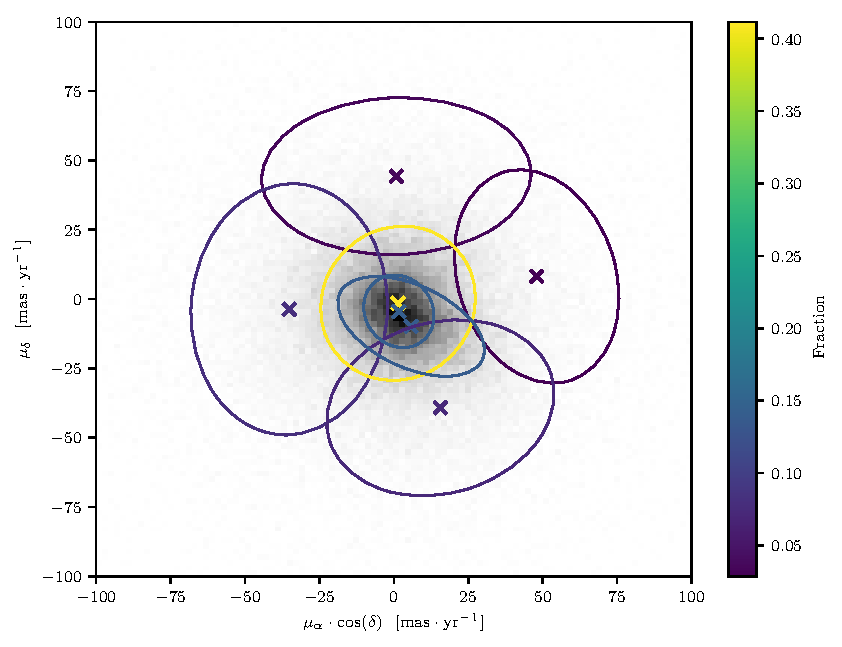
\includegraphics[page=1,width=\textwidth]{background/Figures/GMM-PM-BIC2-U+7G.pdf}
        \caption{}
        \label{fig:fpmMMM} 
    \end{subfigure}
\caption{Gaussian (a) and Modified (b) Mixture Models fitted to the proper motions of the field objects in the RDR2 data set (density in grey scale). The crosses and ellipses indicate the means and the one-$\sigma$ covariance matrices, respectively. The colour code indicates the value of the fraction in the mixture. Uniform distribution not shown in (b)}
\label{fig:GMMvsMMM}
\end{figure}

Finally, the field likelihood $p_f(\mathbf{d}|\boldsymbol{\theta}_f,\mathbf{u})$ of an object with measurements $\mathbf{d}$, given its standard uncertainties $\mathbf{u}$ and the field parameters, $\boldsymbol{\theta}_f$, is
\begin{align}
p_f(\mathbf{d}|\boldsymbol{\theta}_f,\mathbf{u})=&\left[\pi_{f,pm,0}\cdot\mathcal{U}(\textbf{d}_{pm}|S_{\mu_{\alpha}},S_{\mu_{\delta}})+  \sum \limits_{i=1}^{7}\pi_{f,pm,i}\cdot \mathcal{N}(\mathbf{d}_{pm} | \boldsymbol{\mu}_{f,pm,i},\boldsymbol{\Sigma}_{f,pm,i}+\mathbf{u}_{pm})\right]\cdot  \nonumber \\ 
&\left[ \sum \limits_{i=1}^{14}\pi_{f,ph,i}\cdot \mathcal{N}(\mathbf{d}_{ph} | \boldsymbol{\mu}_{f,ph,i},\boldsymbol{\Sigma}_{f,ph,i}+\mathbf{u}_{ph})\right].
\label{eq:field}
\end{align}
The first and second brackets represent the proper motion (subindex $pm$) and photometric (subindex $ph$) models, respectively, with $\boldsymbol{\pi}_f,\boldsymbol{\mu}_f,\boldsymbol{\Sigma}_f$ their fractions, means and covariance matrices, respectively. \textbf{ The first term of the proper motion model is the uniform distribution, with $\pi_{f,pm,0}$ its fraction}. The uncertainty process is convolved (see Section \ref{sect:introprobability}) with the assumed models using the individual proper motions ($\mathbf{u}_{pm}$) and photometric ($\mathbf{u}_{ph}$) uncertainties. 

\subsection{The cluster population}
\label{subsect:cluster}
Similarly to what I assume for the field population model, I also assume that the cluster model or likelihood can be factorised into the product of the proper motions distribution times the photometric distribution. Thus, I assume these two models are independent. 

It is known that unresolved systems of stars (groups of stars that, given the spatial resolution of the telescope, are seen as an individual object) have an increased brightness proportional to the multiplicity of the system. In particular, if an unresolved system is made of two equally luminous objects, then its magnitude is 0.752 times brighter than that of an individual object. This happens for equal mass binaries.

Since the pioneer work of \citet{Trumpler1921}, we know that some of the Pleiades members are double systems. Recently, \citet{Sarro2014} show evidence that some of these double systems lie in an equal-mass binaries (EMB) sequence. Those authors model this EMB sequence assuming that its number of objects is 20\% of the total number of cluster members. In the present work, we also model objects is this displaced EMB sequence  but we do not assume that its proportion is fixed; we infer it from the data. 

Unresolved multiple systems, binary systems particularly, have an impact on the cluster proper motions distribution. In stellar clusters, the massive objects are expected to fall towards the centre of the gravitational potential at a higher rate than that of the less massive ones \textbf{\cite[see for example][p. 556]{Binney2008}}. This behaviour arises from stellar encounters in which the energy exchange results in the less massive objects gaining kinetic energy and the massive ones losing it. \textbf{Since binaries and multiple systems are typically more massive than the average object, they are expected to fall towards the cluster centre.} From an astronomical point of view, an unresolved system shifts the photo-centre of its images when compared to that of a single object. Given the previous considerations, we decide to model the EMB as an independent population in the proper motions. Furthermore, we pair this proper motions model to its photometric counterpart. This more comprehensive statistical model allows us to directly compare the kinematic and photometric properties of the EMB population with those of the rest of the cluster. 

For the sake of simplicity, in the following whenever I refer to the photometric or proper motions model of the EMBs, I call it the EMB sequence model (with the subindex $Bs$). I refer to the model of the rest of the stars as the cluster sequence model or simply single stars. Despite that this is an abuse of the terminology, because there are binaries and multiple systems with different mass ratios, it keeps the text more readable.

\subsubsection{Photometric model of single and EMB stars}

The cluster photometric sequences, both for single and EMB stars, are modelled with cubic splines, one for each of the $Y,J,H,K_s$ vs $CI$ CMDs. I choose the spline series due to their fitting properties. I tried several polynomial bases (monic, Laguerre, Hermite, Chebyshev) but in spite of the order, they were not able to fit the sequence. In specific, they do not fit the region around $CI \sim 3$ where the slope is higher. 

Despite their superior flexibility, spline series require more parameters than polynomials. In addition to the coefficients of the series, they require the specification of points called knots. These knots represent the starting and ending points of the spline sections. 

Any spline function can be represented in terms of basis-splines or B-splines. By definition, a B-spline of order $n$ is a piece-wise polynomial function of order $n$ in the interval $t_0 \leq x \leq t_n$. The boundary and internal points, $\mathbf{t}=\{t_0,t_1,...,t_n\}$ represent the knots. For a given set of knots, there is one and only one B-spline representation of the spline, thus the name basis spline.  In particular, any cubic spline can be represented as,

\begin{equation}
S_3(CI,\boldsymbol{\beta},\mathbf{t}) = \sum_i \beta_i\cdot B_{i,3}(CI,\mathbf{t}).
\end{equation}
Where $B_{i,n}$ are the B-splines given by the Cox-de Boor recursive formula, and $\boldsymbol{\beta}$ are the coefficients of the series. For more details on splines and the Cox-de Boor formula see \citet{deBoor1978}.

Despite their fitting properties, B-splines \textbf{present a problem} when inferring simultaneously their coefficients and knots: there is multi-modality in the parametric space \citep{Lindstrom1999}. It means that at least more than one combination of parameters produces the same solution. To avoid this multi-modality, I decided to keep the knots fixed throughout the inference. Although this decision reduces the flexibility of the splines, it allows a still better fit than that of the tested polynomials. To obtain the maximum-likelihood (ML) estimate of the knots I use the algorithm of  \citet{Spiriti2013}. This algorithm, implemented in the \emph{freeknotsplines} R package, allows to simultaneously obtain the knots and the best truncation value for the spline series. It uses the BIC to select among competing models. In order to obtain both the truncation of the series and the value of the knots, I use the candidate members of \citet{Bouy2015}. The BIC indicates that seven coefficients is the best number of components for the B-spline series, with the knots at $\mathbf{t}=\{0.8,3.22,3.22,5.17,8.0\}$. I tested different number of knots, ranging from two to nine, with five the best configuration given by the BIC. \textbf{In general, the continuity of a spline function is $C^{p-k}$, with $p$ the degree of the spline, and $k$ the highest multiplicity of the knots \citep{deBoor1978}. In our case, since the knot at 3.22 has a multiplicity of two, then the resulting spline has lost one degree of continuity. It is now $C^1$ continuous. It means that the spline and its derivative are continuous, thus ensuring a smooth function.}

As I mentioned in the introduction to this Section, we assume that the observed photometric quantities are drawn from a distribution resulting from the convolution of the observed uncertainties, with the likelihood, given the \emph{true} quantities. We also assume that the model has an intrinsic dispersion that addresses photometric variations resulting from astrophysical phenomena not treated by our model (see Section \ref{sect:parametric_inference}). These phenomena include, but are not limited to, age, metallicity and distance dispersions, unresolved systems (other than EMB), variability, and transits. If we were to assume no \emph{true} intrinsic dispersion, then any deviation from the \emph{true} quantities would have to be explained \emph{only} on the basis of the observational uncertainties. Thus it would result in an over-simplistic model, which would underestimate the likelihood of hypothetical true cluster members. 

This photometric dispersion shows an skewed distribution \cite[see Figure 2 of][which I reproduce in Fig. \ref{fig:luminosity_dispersion}]{2008ASPC..384..200H}, which we model with a multivariate skewed normal distribution \cite[CSN, see for example][]{Gonzalez-Farias2004,Gupta2004}. Despite the fact that the CSN requires only five parameters more than a multivariate normal distribution, the computing of its density takes $\sim$ 50\% more CPU time than that of the multivariate normal distribution (MND). Due to computational constraints, we decided to postpone the results of the CSN until our computational resources allow it. 

Instead of using the CSN, we model the intrinsic photometric  dispersion of both the cluster and EMB sequences with a MND. It has five dimensions corresponding to our photometric reference set: $CI,Y,J,H,K_s$. The B-splines model the \emph{true} photometric quantities, both for the cluster sequence, $\mathbf{t}_{ph;Cs}$, and the EMB, $\mathbf{t}_{ph;Bs}$. The latter is displaced 0.75 into the bright side of the cluster sequence. In the following, the matrix $\Sigma_{clus}$, represents the covariance matrix of this MND. By definition, covariance matrices are symmetric and positive semi-definite. Therefore, from the 25 entries in $\Sigma_{clus}$, only 15 are unique. These are also inferred from the data set.


\begin{figure}[ht!]
\begin{center}
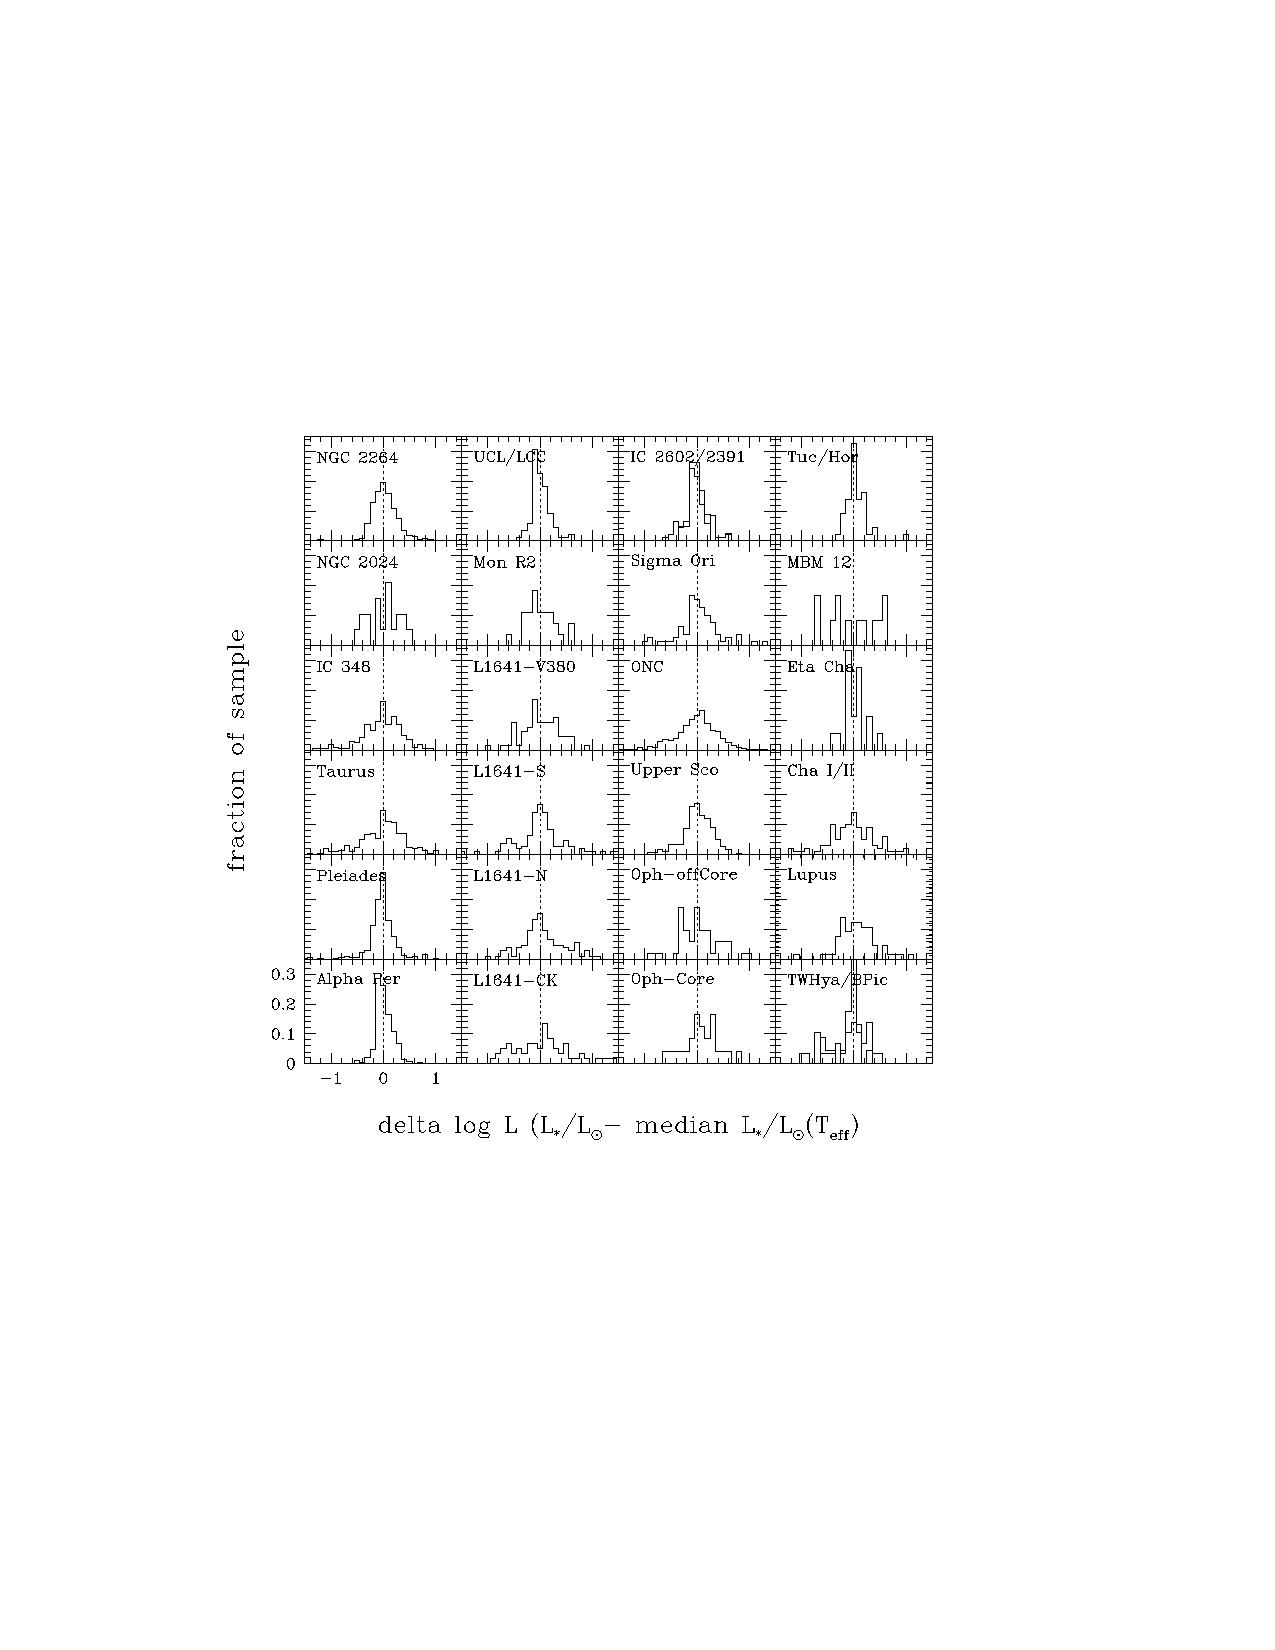
\includegraphics[width=0.8\textwidth]{background/Figures/F2_Hillenbrand2008.pdf}
\caption{Histogram of luminosity dispersion for young clusters. Reproduced from Figure 2 of \citet{2008ASPC..384..200H}, \textit{\usebibentry{2008ASPC..384..200H}{title}}, \usebibentry{2008ASPC..384..200H}{journal}, \usebibentry{2008ASPC..384..200H}{volume}.}
\label{fig:luminosity_dispersion}
\end{center}
\end{figure}


Thus, the \emph{true} photometry is given by,

\begin{align}
\mathbf{t}_{ph;Cs}&= \{CI,Y,J,H,K_s\},\nonumber \\
\mathbf{t}_{ph;Bs}&=\{CI,Y-0.75,J-0.75,H-0.75,K_s-0.75\}, \nonumber
\end{align}
where
\begin{align}
Y &=\mathcal{S}_Y(CI,\hat{\beta}_Y), \nonumber \\
J &=\mathcal{S}_J(CI,\hat{\beta}_J),\nonumber \\
 H &=\mathcal{S}_H(CI,\hat{\beta}_H), \nonumber \\
 K_s &=\mathcal{S}_{K_s}(CI,\hat{\beta}_{K_s}),  \nonumber 
\end{align}
with $\hat{\beta}_{i}, i\in\{Y,J,H,K_s\}$ the vectors of seven coefficients of the B-splines for the $Y,J,H,K_s$ bands.  For the sake of simplicity I denote this $4\times7$ coefficients matrix as $\boldsymbol{\beta}$.

Since the photometry of the EMB is a linear transformation, $T_{Bs}$, of the mean \emph{true} photometry of cluster sequence, no extra parameters are required. Therefore, 

\begin{align}
\mathbf{t}_{ph;Cs} &= \boldsymbol{\mathcal{S}}(CI, \boldsymbol{\beta}) \label{eq:trueph_Cs}\\
\mathbf{t}_{ph;Bs} &=T_{Bs}( \boldsymbol{\mathcal{S}}(CI, \boldsymbol{\beta})).
\label{eq:trueph_Bs}
\end{align}

Thus, cluster and EMB likelihoods of an object with photometric measurements $\mathbf{d}_{ph}$, and standard uncertainties $\mathbf{u}_{ph}$, are:
\begin{align}
\label{eq:lik-seq}
 p_{Cs}(\mathbf{d}_{ph}| CI, \boldsymbol{\beta},\Sigma_{clus},\mathbf{u}_{ph})={\mathcal{N}}(\mathbf{d}_{ph}|\mathbf{t}_{ph;Cs}, \mathbf{u}_{ph}+\Sigma_{clus}),\nonumber \\
p_{Bs}(\mathbf{d}_{ph}| CI, \boldsymbol{\beta},\Sigma_{clus}, \mathbf{u}_{ph})={\mathcal{N}}(\mathbf{d}_{ph}|\mathbf{t}_{ph;Bs}, \mathbf{u}_{ph}+\Sigma_{clus}),
\end{align}
where $\mathbf{t}_{ph;Cs}$ and $\mathbf{t}_{ph;Bs}$ are given by Equations \ref{eq:trueph_Cs} and \ref{eq:trueph_Bs}, respectively.

Since the splines are parametrised by the true $CI$ of each object, we have more parameters than objects in our data set \footnote{Although this sounds crazy, the rules of probability calculus do not discard this possibility.}. This \emph{true} $CI$ is unknown even if its observed value is not missing. We solve this problem (it is a computational problem!) by marginalising these nuisance parameters. 

To marginalise these $CI$s we need a prior, which we provide in a hierarchical way (thus the name Bayesian Hierarchical model). This marginalisation leaves behind a precise estimate of the parameters of the prior distribution. Paradoxically, all objects, even those without a measurement of the $CI$, contribute to this estimate. Here laies the force of the BHM.

\textbf{We model the prior of the \emph{true} $CI$ as a truncated ($0.8\leq CI \leq8$) univariate GMM with five components, whose parameters are also inferred from the data. We choose five components as suggested by the BIC computed from the EM algorithm for GMM applied to the candidate members of \citet{Bouy2015}. I tested larger number of components in the mixture (up to ten), but the posterior distribution did not changed significantly, thus indicating that the BIC value was a proper assumption.}

 The GMM modelling the prior of the \emph{true} $CI$ is 

\begin{equation}
\label{eq:colordist}
p(CI|\boldsymbol{\pi}_{CI},\boldsymbol{\mu}_{CI},\boldsymbol{\sigma}_{CI})= \sum_{i=1}^5 \pi_{CI,i} \cdot \mathcal{N}_t(CI| \mu_{CI,i},\sigma_{CI,i}).
\end{equation}

In this last Equation, the symbol $\mathcal{N}_t$ stands for the truncated ($0.8<CI<8$) univariate normal distribution.

Then, the marginalisation of $CI$ runs as follows:
\begin{align}
\label{eq:clmarginalps}
 p_{Cs}(\mathbf{d}_{ph}| \boldsymbol{\theta}_c,\mathbf{u}_{ph})&=\int p_{Cs}(\mathbf{d}_{ph},CI| \boldsymbol{\theta}_c,\mathbf{u}_{ph}) \cdot \mathrm{d}CI \nonumber \\
 &=\int p_{Cs}(\mathbf{d}_{ph}|CI, \boldsymbol{\theta}_c,\mathbf{u}_{ph}) \cdot p_{Cs}(CI| \boldsymbol{\theta}_c,\mathbf{u}_{ph})\cdot \mathrm{d}CI 
\end{align}
\begin{align}
\label{eq:clmarginalpb}
p_{Bs}(\mathbf{d}_{ph}| \boldsymbol{\theta}_c,\mathbf{u}_{ph})&=\int p_{Bs}(\mathbf{d}_{ph},CI| \boldsymbol{\theta}_c,\mathbf{u}_{ph})\cdot \mathrm{d}CI \nonumber \\
 &=\int p_{Bs}(\mathbf{d}_{ph}|CI, \boldsymbol{\theta}_c,\mathbf{u}_{ph})\cdot p_{Bs}(CI| \boldsymbol{\theta}_c,\mathbf{u}_{ph})\cdot \mathrm{d}CI.
\end{align}
In these Equations, $\boldsymbol{\theta}_c$ stands for all cluster parameters related to photometry, and the first and second terms of the integrals in the last equalities correspond to Equations \ref{eq:lik-seq} and \ref{eq:colordist}, respectively. The distribution of $CI$ depends only on $\boldsymbol{\pi}_{CI},\boldsymbol{\mu}_{CI},\boldsymbol{\sigma}_{CI}$, thus, the cluster and equal-mass binaries likelihoods of datum $\mathbf{d}_{ph}$ are 
\begin{align}
\label{eq:lik-seq2}
 &p_{Cs}(\mathbf{d}_{ph}|\boldsymbol{\pi}_{CI},\boldsymbol{\mu}_{CI},\boldsymbol{\sigma}_{CI},\boldsymbol{\beta},\Sigma_{clus},\mathbf{u}_{ph}) \nonumber \\
 &=\int{\mathcal{N}}(\mathbf{d}_{ph}|\boldsymbol{\mathcal{S}}(CI, \boldsymbol{\beta}), \mathbf{u}_{ph}+\Sigma_{clus})\cdot \sum_{i=1}^5 \pi_{CI,i}\cdot \mathcal{N}_t(CI| \mu_{CI,i},\sigma_{CI,i}) \cdot \mathrm{d}CI\nonumber \\
&p_{Bs}(\mathbf{d}_{ph}|\boldsymbol{\pi}_{CI},\boldsymbol{\mu}_{CI},\boldsymbol{\sigma}_{CI}, \boldsymbol{\beta},\Sigma_{clus}, \mathbf{u}_{ph})\nonumber \\
&=\int{\mathcal{N}}(\mathbf{d}_{ph}|T_{Bs}( \boldsymbol{\mathcal{S}}(CI, \boldsymbol{\beta})), \mathbf{u}_{ph}+\Sigma_{clus}) \cdot \sum_{i=1}^5 \pi_{CI,i}\cdot \mathcal{N}_t(CI| \mu_{CI,i},\sigma_{CI,i}) \cdot \mathrm{d}CI.
\end{align}

The observed $CI$ and magnitudes help us  to reduce the computing time of the marginalisation integral. We use them to discard  regions of the integral in which the argument is almost zero (i.e. far from the measured values). Although we allow the nuisance parameters $CI$s to have all their possible values, the data, by means of the likelihood, give us information about the distribution of these individual nuisance parameters. To use this information, we proceed as follows. First, we compare the observed photometry to the true one (i.e. the cluster sequence given by the splines). For it we use a grid of 300 points uniformly distributed in the domain of $CI$ ($0.8<CI<8$)\footnote{\label{foot:extendedCI}As explained in Section \ref{sect:RDR2}, if this $CI$ range will have covered that of all the objects in the DANCe DR2 data set, the marginalisation integral would have to be computed over the extended $CI$ range. Therefore, the computing time of the BHM would have also increased proportionally to the number of extra points in this integral.}. Then, we find the point, $p$, of the grid that is closest to the vector of the observed photometry.  Distance is computed under  the Mahalanobis metric. This metric takes into account the observational uncertainty, $\mathbf{u}_{ph}$, and the intrinsic dispersion of the cluster sequence, $\Sigma_{clus}$. Finally, the limits of the marginalisation integral  are defined as those given by a ball of 3.5 Mahalanobis distances around point $p$. Contributions outside this ball are negligible to the integral ($< 4\times10^{-4}$).

\subsubsection{Proper motion model of EMB and single stars}
As mentioned before, we assume that the cluster population has two subpopulations: single and EMB stars.
We model the proper motions of these two subpopulations with independent GMM. If the cluster is virialised (see Chapter \ref{chap:pleiades}), we can assume that\textbf{ the distribution of its velocity modulus} is almost Maxwellian (Maxwell-Boltzman distribution). Therefore a GMM is a reasonable \textbf{approximation}. Furthermore, in the absence of external forces, a virialised system is expected to have spherical symmetry both in its spatial and velocity distributions. Thus we can safely assume that the gaussians within each GMM are concentric, thus they share the same mean. However we allow independent means for both single and EMB subpopulations. The assumption of spherical symmetry may be a weak one in the presence of the galactic potential. It can perturb the cluster and deviate its spatial and velocity distribution from spherical symmetry. Furthermore, the ellipticity of the spatial distribution, which has been reported to be no-negligible \cite[$\epsilon=0.17$, according to ][]{Raboud1998}, can be due to projection effects that further deviate the observed velocity distribution profile from spherical symmetry. Nevertheless, since we model the covariance matrices of the GMM of both single and EMB, as full covariance matrices, any departure from the spherical symmetry in the velocity distribution can still be modelled by the non-diagonal entries of these matrices.


We infer the parameters of these GMMs as part of our Bayesian hierarchical model. However we set a priori the number of gaussians in each GMM. Not doing so will demand a technique in which the model parameters can be augmented. Although such techniques already exist, they are still under computational development \cite[see][for a review of reversible jump MCMC]{Fan2011}.

Using the EM algorithm for GMM and the proper motions of the candidate members of \citet{Bouy2015}, I obtained the ML estimates for the GMM likelihoods. I did this for configurations of GMM ranging from one to five components. The BIC (Eq. \ref{eq:BIC}) suggested four and two components for the cluster and EMB GMMs, respectively. Since covariance matrices are always symmetric, only three parameters are needed to fully specify the covariance matrices of these bivariate normal distributions.

The cluster (subindex $Cs$) and EMB (subindex $Bs$) likelihoods of an object with proper motions measurements $\mathbf{d}_{pm}$, and uncertainties $\mathbf{u}_{pm}$, are

\begin{align}
p_{Cs}(\mathbf{d}_{pm}| \boldsymbol{\pi}_{Cs}, \boldsymbol{\mu}_{Cs},\boldsymbol{\Sigma}_{Cs},\mathbf{u}_{pm})
&= \sum_{i=1}^4\pi_{Cs,i}\cdot \mathcal{N}(\mathbf{d}_{pm} | \boldsymbol{\mu}_{Cs},\Sigma_{Cs,i}+\mathbf{u}_{pm}) \nonumber\\
p_{Bs}(\mathbf{d}_{pm}| \boldsymbol{\pi}_{Bs}, \boldsymbol{\mu}_{Bs},\boldsymbol{\Sigma}_{Bs},\mathbf{u}_{pm})
&= \sum_{i=1}^2\pi_{Bs,i}\cdot \mathcal{N}(\mathbf{d}_{pm} | \boldsymbol{\mu}_{Bs},\Sigma_{Bs,i}+\mathbf{u}_{pm}).
\label{eq:lik-pm}
\end{align}

Finally, combining the proper motions and photometric models, the total cluster likelihood of an object with measurement $\mathbf{d}$, and uncertainties $\mathbf{u}$, is

\begin{align}
p_c(\mathbf{d}|\boldsymbol{\theta}_c,\mathbf{u})=\pi_{CB}&\cdot p_{Cs}(\mathbf{d}_{pm}| \boldsymbol{\pi}_{Cs}, \boldsymbol{\mu}_{Cs},\boldsymbol{\Sigma}_{Cs},\mathbf{u}_{pm}) \cdot  p_{Cs}(\mathbf{d}_{ph}|\boldsymbol{\pi}_{CI},\boldsymbol{\mu}_{CI},\boldsymbol{\sigma}_{CI},\boldsymbol{\beta},\Sigma_{clus},\mathbf{u}_{ph})\nonumber\\
+(1-\pi_{CB})&\cdot p_{Bs}(\mathbf{d}_{pm}| \boldsymbol{\pi}_{Bs}, \boldsymbol{\mu}_{Bs},\boldsymbol{\Sigma}_{Bs},\mathbf{u}_{pm}) \cdot  p_{Bs}(\mathbf{d}_{ph}|\boldsymbol{\pi}_{CI},\boldsymbol{\mu}_{CI},\boldsymbol{\sigma}_{CI}, \boldsymbol{\beta},\Sigma_{clus}, \mathbf{u}_{ph}),
\end{align}

where $\pi_{CB}$ is the parameter representing the proportion or fraction of single cluster sequence stars in the single-EMB mixture model. The photometric and proper motions likelihoods are given by Equations \ref{eq:lik-seq2} and \ref{eq:lik-pm}, respectively.

Finally, before ending this Section, I present a summary of the symbols used to represent the parameters in the BHM (Table \ref{tab:symbols_parameters}), together with its graphical representation in the form of a PGM (Fig. \ref{fig:PGMBHM}).
\input{background/Tables/SymbolParameters.txt}


\begin{figure}[H]
  \begin{center}
  \resizebox{0.8\textwidth}{!}{
%\documentclass[12pt]{amsart}
%\usepackage{bm}
%\usepackage{color}
%\usepackage[usenames,dvipsnames,svgnames,table]{xcolor}
%\usepackage{tikz}
%\usetikzlibrary{arrows,arrows.meta,shapes,decorations.pathmorphing,positioning,intersections,calc,backgrounds}
\tikzstyle{line} = [draw, -latex']
\tikzstyle{marginalized}=[black, {Circle[color=black,length=3pt]-latex[]}]
%\tikzstyle{con} = [thick, dashed, draw, angle 90 reversed-angle 90 reversed]
%\tikzset{
%    box1/.style={%
%        draw=black, thick,
%        rectangle,
%        rounded corners,
%        minimum height=4cm,
%        minimum width=4cm
%    },
%    snake arrow/.style=
%{->,
%decorate,
%decoration={snake,amplitude=.4mm,segment length=2mm,post length=1mm}}
%}
%
%
%% See the ``Article customise'' template for come common customisations
%
%%%% BEGIN DOCUMENT
%\begin{document}
%\begin{figure}[tb]
%  \begin{center}
%  \resizebox{0.9\linewidth}{!}{
\begin{tikzpicture}[>=stealth', node distance = 1cm, every node/.style={rectangle,fill=white}]

%############### Principal block ###################
% Variables 
\node[draw, fill = gray!20, circle, label={[name=x_i_lab,xshift=-10pt,yshift=3pt]below:$\boldsymbol{d}$}] (x_i) at (0,0) {$[7]$};
\node[draw, circle, label={[name=pi_lab,xshift=-10pt,yshift=3pt]below:$\pi$}] (pi) [above = of x_i] {$[1]$};
\node[draw, fill = gray!20, label={[name= alpha_lab]above:$\boldsymbol{\alpha}$}] (alpha) [above = of pi] {$[2]$};

% relations
\path[line] (alpha) -> (pi);
\draw[marginalized] (pi) -- (x_i);
% plates
\begin{pgfonlayer}{background}
\node (rect) at (x_i) [xshift = 0pt, yshift = -3pt, draw, rounded corners, thick, minimum width=50pt, 
minimum height=50pt, line width=1pt, fill=yellow!90!blue, fill opacity=0.3] (rect1) {};
\end{pgfonlayer}
\node[anchor=south east,inner sep=5pt, fill = none] at (rect1.south east) {$N$};

%############# NON-MEMBERS ##############################
\node[draw, fill = gray!20, label={[name = mu_nm_pm_lab,xshift=0pt,yshift=2pt]above:$\boldsymbol{\mu}_{f,pm}$}] (mu_nm_pm) [left = of x_i,xshift=-120pt,yshift=100pt] {$[2]$};

\node[draw, fill = gray!20, label={[name = sg_nm_pm_lab,xshift=0pt,yshift=2pt]above:$\Sigma_{f,pm}$}] (sg_nm_pm) [right = of mu_nm_pm,yshift=0pt] {$[2,2]$};
\node[draw, fill = gray!20, label={[name = pi_nm_pm_lab,xshift=0pt,yshift=0pt]above:$\pi_{f,pm}$}] (pi_nm_pm) [right = of sg_nm_pm,xshift=5pt,yshift=0pt] {[8]};

\node[draw, fill = gray!20, label={[name = mu_nm_phot_lab,xshift=0pt,yshift=2pt]below:$\boldsymbol{\mu}_{f,ph}$}] (mu_nm_phot) [left = of x_i,xshift=-120pt,yshift=-60pt] {$[5]$};

\node[draw, fill = gray!20, label={[name = sg_nm_phot_lab,xshift=0pt,yshift=2pt]below:$\Sigma_{f,ph}$}] (sg_nm_phot) [right = of mu_nm_phot,yshift=0pt] {$[5,5]$};
\node[draw, fill = gray!20, label={[name = pi_nm_phot_lab,xshift=0pt,yshift=0pt]below:$\pi_{f,ph}$}] (pi_nm_phot) [right = of sg_nm_phot,xshift=5pt,yshift=0pt] {[14]};


\begin{pgfonlayer}{background}
\node (rect) at (mu_nm_pm) [xshift = 35pt, yshift = 5pt, draw, rounded corners, thick, minimum width=110pt, 
minimum height=50pt, line width=1pt, fill=gray!20, fill opacity=0.5] (rect2) {};
\end{pgfonlayer}
\node[anchor=south east,inner sep=5pt, fill = none] at (rect2.south east) {7};

\begin{pgfonlayer}{background}
\node (rect) at (mu_nm_phot) [xshift = 35pt, yshift = -4pt, draw, rounded corners, thick, minimum width=110pt, 
minimum height=50pt, line width=1pt, fill=gray!20, fill opacity=0.5] (rect2) {};
\end{pgfonlayer}
\node[anchor=south east,inner sep=5pt, fill = none] at (rect2.south east) {14};

\draw [->,name path=curve] (mu_nm_pm) to [out = -90, in = 180, looseness=1] (x_i);
\draw [->,name path=curve] (sg_nm_pm) to [out = -90, in = 180, looseness=1] (x_i);
\draw [->,name path=curve] (pi_nm_pm) to [out = -90, in = 180, looseness=1] (x_i);

\draw [->,name path=curve] (mu_nm_phot) to [out = 90, in = 180, looseness=1] (x_i);
\draw [->,name path=curve] (sg_nm_phot) to [out = 90, in = 180, looseness=1] (x_i);
\draw [->,name path=curve] (pi_nm_phot) to [out = 90, in = 180, looseness=1] (x_i);
%############# MEMBERS ##############################
% photometry block
\node[draw, circle, label={[name = t_phot_lab,xshift=-10pt,yshift=3pt]below:$$}] (t_phot) [right = of x_i,xshift=100pt,yshift=25] {$\boldsymbol{t}_{ph}$};
\node[draw, circle, label={[name = idx_clr_lab,xshift=-10pt,yshift=3pt]below:$$}] (idx_clr)  [above = of t_phot]  {$CI$};
\node[draw, circle, label={[name = sg_phot_lab,xshift=-10pt,yshift=3pt]below:$\Sigma_{clus}$}] (sg_phot) [left = of idx_clr,xshift=10pt] {$[15]$};
\node[draw, circle, label={[name = pi_phot_lab,xshift=-15pt,yshift=3pt]below:$\pi_{CB}$}] (pi_phot) [below= of x_i, xshift=0pt,yshift=-0pt] {$[1]$};
\node[draw, circle, label={[name = beta_lab,xshift=-10pt,yshift=3pt]below:$\boldsymbol{\beta}$}] (beta) [right = of idx_clr] {$[4,7]$};
\node[draw, circle, label={[name = mu_clr_lab,xshift=-10pt,yshift=3pt]below:$\mu_{CI}$}] (mu_clr) [above = of idx_clr] {$[1]$};
\node[draw, circle, label={[name = pi_clr_lab,xshift=-10pt,yshift=3pt]below:$\pi_{CI}$}] (pi_clr)  [left = of mu_clr]  {$[4]$};
\node[draw, circle, label={[name = sigma_clr_lab,xshift=-5pt,yshift=3pt]below:$\sigma_{CI}$}] (sigma_clr) [right = of mu_clr ]{$[1]$};

\draw (idx_clr)  node[fill=none,minimum size=16pt,draw] {};

\node[draw, fill = gray!20, label={[name = mu_beta_lab]above:$\boldsymbol{\mu}_{\beta}$}] (mu_beta) [right = of beta]{$[4,7]$};
\node[draw, fill = gray!20, label={[name = sg_beta_lab]above:$\boldsymbol{\sigma}_{\beta}$}] (sg_beta) [above = of mu_beta] {$[7]$};
\node[draw, fill = gray!20, label=below:$\boldsymbol{\alpha}_{CB}$] (alpha_phot) [below=of pi_phot] {$[2]$};
\node[draw, fill = gray!20, label={[name = alpha_clr_0_lab]above:$\boldsymbol{\alpha}_{CI}$}] (alpha_clr_0) [above = of pi_clr] {$[5]$};
\node[draw, fill = gray!20, label={[name = rg_clr_lab]above:$rg_{CI}$}] (rg_clr) [above = of mu_clr,xshift=0pt] {$[2]$};
\node[draw, fill = gray!20, label={[name = eta_clr_lab]above:$\eta$}] (eta_clr) [above = of sigma_clr,xshift=0pt] {$[1]$};
\node[draw, fill = gray!20, label={[name = nu_phot_lab]above:$\nu$}] (nu_phot) [left = of sg_phot,yshift=0pt] {$[1]$};
\node[draw, fill = gray!20, label={[name = A_phot_lab]above:$\boldsymbol{A}_{ph}$}] (A_phot) [above = of nu_phot,yshift=0pt] {$[5]$};
\begin{pgfonlayer}{background}
\node (rect) at (idx_clr) [xshift = 0pt, yshift = 25pt, draw, rounded corners, thick, minimum width=170pt,
 minimum height=120pt, line width=1pt, fill=black!20!red, fill opacity=0.5] (rect4) {};
\end{pgfonlayer}

\begin{pgfonlayer}{background}
\node (rect) at (mu_clr) [xshift = 30pt, yshift = -5pt, draw, rounded corners, thick, minimum width=100pt,
 minimum height=60pt, line width=1pt, fill=none] (rect5) {};
\end{pgfonlayer}
\node[anchor=south east,inner sep=5pt, fill=none] at (rect5.south east) {$5$};


\path [line,dashed] (idx_clr) -> (t_phot);
\path [line,dashed] (beta) -> (t_phot);
\path[line] (mu_clr) -> (idx_clr);
\path[line] (sigma_clr) -> (idx_clr);
\draw[marginalized] (pi_clr) to (idx_clr);
\path[line] (mu_beta) -> (beta);
\path[line] (sg_beta) -> (beta);
\path[line] (alpha_clr_0) -> (pi_clr);
\path[line] (rg_clr) -> (mu_clr);
\path[line] (eta_clr) -> (sigma_clr);
\path[line] (alpha_phot) -> (pi_phot);
\path[line] (A_phot) -> (sg_phot);
\path[line] (nu_phot) -> (sg_phot);

\draw [marginalized,name path=curve] (pi_phot) to [out = 0, in = 0, looseness=2] (x_i);
\draw [name path=curve] (t_phot) to [out=180,in=0, looseness=1.0]  (x_i);
\draw [name path=curve] (sg_phot) to [out = 270, in = 0, looseness=1.0] (x_i);

% propermotion block
%----singles --------
\node[draw, circle, label={[name = pi_pm_lab,xshift=-10pt,yshift=3pt]below:$\boldsymbol{\pi}_{Cs}$}] (pi_cs) [below= of t_phot,xshift=-55pt]{$[3]$};
\node[draw, circle, label={[name=mu_pm_lab,xshift=-10pt,yshift=3pt]below:$\boldsymbol{\mu}_{Cs}$}] (mu_cs) [below= of pi_cs] {$[2]$};
\node[draw, circle, label={[name = sigma_pm_lab,xshift=-10pt,yshift=3pt]below:$\Sigma_{Cs}$}] (sigma_cs) [below = of mu_cs] {$[3]$};

\begin{pgfonlayer}{background}
\node (rect) at (sigma_cs) [xshift = 0pt, yshift = -0pt, draw, rounded corners, thick, minimum width=50pt,
 minimum height=55pt, line width=1pt, fill=none] (rect3) {};
\end{pgfonlayer}
\node[anchor=south east,inner sep=5pt, fill = none] at (rect3.south east) {$4$};

\begin{pgfonlayer}{background}
\node (rect) at (mu_cs) [xshift = 0pt, yshift = -10pt, draw, rounded corners, thick, minimum width=60pt,
 minimum height=170pt, line width=1pt, fill=gray!50!blue,fill opacity=0.3] (rect3) {};
\end{pgfonlayer}
%-------binaries -----------
\node[draw, circle, label={[name = pi_pm_lab,xshift=-10pt,yshift=3pt]below:$\boldsymbol{\pi}_{Bs}$}] (pi_bs) [below= of t_phot,xshift=55pt]{$[1]$};
\node[draw, circle, label={[name=mu_pm_lab,xshift=-10pt,yshift=3pt]below:$\boldsymbol{\mu}_{Bs}$}] (mu_bs) [below= of pi_bs] {$[2]$};
\node[draw, circle, label={[name = sigma_pm_lab,xshift=-10pt,yshift=3pt]below:$\Sigma_{Bs}$}] (sigma_bs) [below = of mu_bs] {$[3]$};

\begin{pgfonlayer}{background}
\node (rect) at (sigma_bs) [xshift = 0pt, yshift = -0pt, draw, rounded corners, thick, minimum width=50pt,
 minimum height=55pt, line width=1pt, fill=none] (rect3) {};
\end{pgfonlayer}
\node[anchor=south east,inner sep=5pt, fill = none] at (rect3.south east) {$2$};

\begin{pgfonlayer}{background}
\node (rect) at (mu_bs) [xshift = 0pt, yshift = -10pt, draw, rounded corners, thick, minimum width=60pt,
 minimum height=170pt, line width=1pt, fill=green!50!blue,fill opacity=0.3] (rect3) {};
\end{pgfonlayer}
%-------- hyper parameters


\node[draw, fill = gray!20, label={[name = mu_pm_lab]below:$\boldsymbol{\mu}_{\mu_{pm}}$}] (mu_pm) [below= of t_phot,yshift=-34pt] {$[2]$};
\node[draw, fill = gray!20, label={[name = sg_pm_lab]below:$\Sigma_{\mu_{pm}}$}] (sg_pm) [below = of mu_pm,yshift=15pt] {$[2,2]$};

\node[draw, fill = gray!20, label={[name = nu_pm_lab]below:$\nu$}] (nu_pm) [below = of sg_pm,yshift=10pt] {$[1]$};
\node[draw, fill = gray!20, label={[name = A_pm_lab]below:$\boldsymbol{A}_{pm}$}] (A_pm) [below = of nu_pm,yshift=15pt] {$[2]$};


\node[draw, fill = gray!20, label=below:$\boldsymbol{\alpha}_{Cs}$] (alpha_cs) [right=of pi_cs,xshift=-10pt,yshift=5pt] {$[4]$};
\node[draw, fill = gray!20, label=below:$\boldsymbol{\alpha}_{Bs}$] (alpha_bs) [left=of pi_bs,xshift=10pt,yshift=5pt] {$[2]$};
 
\draw [marginalized,name path=curve] (pi_cs) to [out = 150, in = 0, looseness=1] (x_i);
\draw [name path=curve] (mu_cs) to [out = 120, in = 0, looseness=0.8] (x_i);
\draw [name path=curve] (sigma_cs) to [out = 120, in = 0, looseness=0.9] (x_i);

\draw [marginalized,name path=curve] (pi_bs) to [out = 150, in = 0, looseness=1] (x_i);
\draw [name path=curve] (mu_bs) to [out = 60, in = 0, looseness=1.5] (x_i);
\draw [name path=curve] (sigma_bs) to [out = 70, in = 0, looseness=2] (x_i);

\path[line] (alpha_cs) -> (pi_cs);
\path[line] (mu_pm) -> (mu_cs);
\path[line] (sg_pm) -> (mu_cs);
\path[line] (A_pm) -> (sigma_cs);
\path[line] (nu_pm) -> (sigma_cs);

\path[line] (alpha_bs) -> (pi_bs);
\path[line] (mu_pm) -> (mu_bs);
\path[line] (sg_pm) -> (mu_bs);
\path[line] (A_pm) -> (sigma_bs);
\path[line] (nu_pm) -> (sigma_bs);

\end{tikzpicture}
%}\end{center}
%\end{figure}
%\end{document}}
  \end{center}
  \caption{Probabilistic graphical model representing the BHM. The left grey plates show the field model. The middle yellow plate shows the node where the likelihood is computed for each datum, $\boldsymbol{d}$. The right plates describe the relations among parameters in the cluster model. The photometric cluster model (red) is on top, while the proper motions cluster (blue) and equal-mass binaries (green) are at the bottom left and right, respectively. See Section \ref{sect:PGM} for more details. Reproduced from Figure 19 of \citet{Olivares2017},\textit{\usebibentry{Olivares2017}{title}}, \usebibentry{Olivares2017}{journal}, \usebibentry{Olivares2017}{volume}.}
  \label{fig:PGMBHM}
\end{figure}

\section{The methodology for the analysis of the PSD}
\label{sect:PSDmethod}

In this Section, I present the methodology applied to investigate the Projected Spatial Distribution (PSD). This analysis is independent of that of the performed by the BHM using the kinematic and photometric observables. The reasons of this decision are detailed in Section \ref{sect:RF-2}. 

The generative model of the PSD is similar to that of Eq. \ref{eq:genmod}. However, instead of inferring the fraction of field objects in the data set (which would be similar to the estimated contamination rate on the HMPS, see Section \ref{sect:classifier}), each object contributes to the cluster model proportionally to its membership probability, $P$. Thus the generative model of the PSD for object $n$ is

\begin{equation}
\label{eq:genmodPSD}
p(\mathbf{d}_n, P_n |\boldsymbol{\theta}_c,\boldsymbol{\theta}_f)=(1-P_n) \cdot p_f(\mathbf{d}_n|\boldsymbol{\theta}_f) + P_n\cdot p_c(\mathbf{d}_n| \boldsymbol{\theta}_c),
\end{equation}

with $\mathbf{d}_n$ its vector of observations, comprising the right ascension $\alpha$ (R.A.) and the declination $\delta$ (Dec.), and $P_n$ its cluster membership probability. The terms $p_f(\mathbf{d}_n|\boldsymbol{\theta}_f)$ and $p_c(\mathbf{d}_n|\boldsymbol{\theta}_c)$ are the field and cluster likelihood of datum $\mathbf{d}_n$ given the field, $\boldsymbol{\theta}_f$ and cluster, $\boldsymbol{\theta}_c$, parameters. Since all objects in the Pleiades DANCe DR2 have R.A. and Dec. uncertainties which are symmetric, almost identical, and negligible ($\sim 2\times10^{-6}$ deg) compared to the size of the cluster ($\sim7^{\circ}$), we can safely assume that: i) the data are independent and identically distributed, and ii) the contributions of the uncertainties to the models are negligible. 

We would expect that the fraction of contaminants in the HPMS will be uniformly distributed in right ascension and declination because the position on the sky was explicitly removed from the calculation of membership probabilities. Except perhaps for a mild positive gradient of the density towards the Galactic centre. Hence, we model of these contaminants with a uniform spatial distribution $\mathcal{U}$. In this way, the contribution of these hypothetical contaminants will not bias our inference of the cluster parameters.

In the following Section, I describe the two kind of PSD models that we included in our model selection analysis: those with radial symmetry, and those with luminosity segregation (a proxy for mass segregation). The former are the classical ones in the literature. The latter allow us to put a solid statistical background to the assumption of mass segregation in the Pleiades cluster \cite[see for example][]{2004A&A...426...75M, Converse2010} without relying on mass-luminosity transformations for individual objects. 

\subsection{Models with radial symmetry}
The first alternative is King profile \citep{King1962}, which has been widely used in the Pleiades (see Section \ref{}) and to describe open clusters
\citep[see][for recent applications]{2017MNRAS.469.1330A,2017MNRAS.468.2684P}, globular clusters \citep{2017MNRAS.468.4513M} and even to study
galaxies \citep{2017MNRAS.466.1513R}, halo substructure \citep{2007ApJ...663..960S} and the dark matter distribution \citep{2016MNRAS.458.2848J}. 

The analytical description of the surface number density of stars counts $n$ is given by

\begin{equation}
  \rho(R) = k\cdot\left(\frac{1}{\sqrt{[1+(R/R_c)^2}}-\frac{1}{\sqrt{[1+(R_t/R_c)^2]}}\right)^2
\end{equation}

where $R_c$ (the core radius) is a scale factor, $R_t$ is the tidal radius, and $k$ is a constant related (but not equal) to the central surface density. In the following we use $R$ instead of $r$ (as is often common in some of the articles that introduced the profile analytic expressions used here) to refer to the distance from the system centre projected on the celestial sphere. Also, we use $\rho$ to denote the surface number density of stars, and $I$ to refer to the projected surface brightness.

We have also considered the model proposed by \cite{EFF1987} (henceforth EFF) to describe young open clusters in the Large Magellanic Cloud. Their surface density (in star counts per solid angle) is given by

\begin{equation}
\rho(R)=\rho(0)\cdot(1+(R^2/A^2))^\frac{\gamma}{2}.
\label{eq:eff}
\end{equation}

Equation \ref{eq:eff} is introduced heuristically and hence, the two parameters $A$ and $\gamma$ have no physical meaning (although $A$ must have the same units as $R$).

Finally, we analyse a more general parameterization introduced in \cite{1995AJ....110.2622L}, \cite{1996AJ....111.1889B} and \cite{Zhao1997}, where the projected mass density is given as

\begin{equation}
  \rho(R) = \frac{k'}{(R/R_b)^{\gamma}\cdot(1+(R/R_b)^{1/\alpha})^{(\gamma-\beta)\alpha}}.
  \label{eq:zhao}
\end{equation}

Equation \ref{eq:zhao} represents a double power law with $\gamma$ being the exponent in the innermost region, $\beta$ the exponent in the outer region, $\alpha$ is the width of the transition region, $R_b$ is the so called break radius, and $k'$ is a scale constant. In purity, the aforementioned works assume this functional form for both the projected surface brightness $I$, the projected mass density $\rho$, and for the volume density $v$, although the latter two are related by integration:

\begin{equation}
  \rho(R) = \int_{0}^{\infty}v(r)\cdot {\rm d}z  
\end{equation}

where $z$ is the distance along the line of sight corresponding to a radial distance projected onto the plane of the sky $R$.

In this work we will assume that the analytical expression in Eq. \ref{eq:zhao} is correctly stated in terms of the number density and not of volume density.

This model is a more general analytical expression that comprises many simpler models each of which represent particular choices of the model parameters. For example, the model put forward by \cite{1911MNRAS..71..460P} to describe the projected spatial density corresponds to the general model with $\alpha=1/2$, $\beta=5$ and $\gamma=0$. Several density profiles proposed to describe galaxies can be grouped by particular choices of the parameters. For example, $\alpha=1$ includes models by \cite{1997ApJ...490..493N}, \cite{1990ApJ...356..359H},\cite{1983MNRAS.202..995J}, and \cite{1999MNRAS.310.1147M}, and $\alpha=1/2, \gamma=0$ includes the aforementioned model by \cite{1911MNRAS..71..460P}, and also models by \cite{1990ApJ...361..408S} and \cite{1985MNRAS.216..273D}. King's profile, however, cannot be cast into this general model unless the tidal radius $R_t$ is fixed at infinity. This is an important difference that will nevertheless have little effect on our comparisons for reasons that will become apparent further below.

In all three cases, we need to convert the projected stellar densities (number of stars per unit solid angle) into probability density functions that describe the probability of finding a star between $R$ and $R+{\rm d}R$ under the assumption of spherical symmetry. In all three cases we can construct the probability densities from their definitions:

\begin{equation}
\rho(R)=\frac{N\cdot p(R)\cdot {\rm d}R}{2\pi\cdot R\cdot {\rm d}R}
\label{eq:probfromdens}
\end{equation}

where $N$ is the total number of stars in the system. Applying Equation \ref{eq:probfromdens} to King's profile, we obtain

\begin{equation}
  p(R)=\frac{k\cdot2\pi}{N}\cdot r \cdot
  \left(\frac{1}{\sqrt{1+(R/r_c)^2}} - \frac{1}{\sqrt{1+(r_c/r_t)^2}}\right)^2
\end{equation}

Actually, in probabilistic inference we write this probability function as:

\begin{equation}
  p(R|r_c, r_t, k_1,\mathcal{M}_1)=k_1\cdot r \cdot
  \left(\frac{1}{\sqrt{1+(R/r_c)^2}} - \frac{1}{\sqrt{1+(r_c/r_t)^2}}\right)^2
\label{eq:probfromdens1}
\end{equation}

where we have defined a new constant $k_1=\frac{k\cdot2\pi}{N}$, and made explicit the dependence of the probability on the underlying analytical expression ($\mathcal{M}_1$), and the values of the parameter set ($k_1, r_c and r_t$). In practice $k_1$ is treated as a normalisation constant (to enforce unit integral) and there is no need to know the total number of stars in the system. This probability density for a given model and parameter set is known in the statistical jargon as {\it likelihood}.

Likewise, the expression for the EFF model is

\begin{equation}
  p(R|a, \gamma, k_2,\mathcal{M}_2)=k_2\cdot r \cdot (1+(R^2/a^2))^\frac{\gamma}{2}.
\label{eq:probfromdens2}
\end{equation}

And finally, the generic model will be given by

\begin{equation}
  p(R| \alpha, \beta, \gamma, R_b, k_3,\mathcal{M}_3 ) = \frac{k_3\cdot r} {(R/R_b)^{\gamma}\cdot(1+(R/R_b)^{1/\alpha})^{(\gamma-\beta)\alpha}}.
  \label{eq:probfromdens3}
\end{equation}

In all three cases, the $R$ coordinate is defined with respect to the origin of a coordinate axis. The actual values of $R$ then depend on this choice of origin. We therefore infer this centre as part of our models in order to incorporate all sources of uncertainty. 


\subsubsection{Extensions of the classical profiles}

In addition to the classical profiles we have tested two extensions of the King profile, and one variant of the generalised profile. Let us describe them in order.

We define the generalised King profile (hereafter GKing profile) as the classical King profile without fixing the exponents of the analytical expression. Instead of Equation \ref{eq:probfromdens1}, we have

\begin{multline}
%\begin{eqnarray}
%\begin{split}
  p(R|r_c, r_t, k_1,\mathcal{M}_1)=\\
  k_1\cdot r \cdot
  \left(
  \left(1+(R/r_c)^{\frac{1}{\alpha_1}}\right)^{-\alpha_1}
  -
  \left(1+(r_c/r_t)^{\frac{1}{\alpha_1}}\right)^{-\alpha_1}
  \right)^{\alpha_2}\\
%  \end{split}
\label{eq:GKing}
%\end{eqnarray}
\end{multline}

where the classical King's profile is recovered for $\alpha_1=2$ and $\alpha_2=2$.

The optimized/generalized King profile (hereafter OGKing) is the GKing profile with the values of $\alpha_1$ and $\alpha_2$ fixed so as to maximise the evidence evaluated with all DANCe DR2 sources. The reasons for this will become apparent after Section \ref{sec:modelselect}, but we can write here that this choice is the most favourable for the GKing profile in the context of model selection.

Finally, the restricted/generalised profile (RGP) corresponds to the generalised profile with the value $\gamma$ fixed at 0.


% HERE
% tomorrow: elliptical profile, luminosity segregation
% and start describing the results

\subsection{Central symmetry constraint}

So far, we have defined a set of three models (King, EFF and the
generalised profile GP) and their extensions. Each has a different set
of parameters.  King's model depends on two parameters ($r_c$ and
$r_t$); EFF's model depends on two parameters ($a$ and $\gamma$); the
generalised profile depends on four parameters ($\alpha$, $\beta$, $\gamma$
and $R_b$).

In reality, there are always two more parameters that do not appear
explicitly in any of the classical analytical formulations of the
King, EFF or generalised profiles. These are the cluster center
coordinates from which all radial distances $r_i$ are measured. It is
not a minor question because the problem is degenerate, and there is a
maximum likelihood solution for each choice of the cluster center. In
principle, one could even choose a poor cluster center estimate that
renders the angular distribution of members asymmetric, and obtain
a maximum likelihood fit better than those obtained with a better
centred estimate.  The models assume central symmetry, but this can
only be ensured approximately. There is a region of non-negligible
extent, where the cluster center may be, and any particular choice of
its position will influence the posterior distribution inferred. Thus,
in order to propagate appropriately this uncertainty about the cluster
center position in our posterior inferences, we have included the two
cluster centre coordinates as further parameters of our models.

The requirement of central symmetry is enforced by the inclusion of a
multiplicative term in the likelihood. The new likelihood term is
based on the empirical distribution function and is expressed as

\begin{equation}
\mathcal{L}(\bm{\phi}) = p(\bm{\phi}|\bm{\theta}) = \prod_{n=1}^{N}\mathcal{N}(\phi_n|\mu=n\cdot2\pi/N,\sigma)
\end{equation}

where $\bm{\phi}$ is the vector of ordered angles $\phi_n\in {0,2\pi}$
calculated for a given centre and coordinate system (parameters
included in the set $\bm{\theta}$); $\phi_n$ is the n-th angle in the
vector $\bm{\phi}$, and $\sigma$ is the allowed level of departure
from the cumulative distribution function of the uniform distribution.
For any given choice of the cluster centre coordinates $\alpha_c$ and
$\delta_c$ we calculate the position angle \citep[using the four-parts
formula given in p. 12 of ]{1985spas.book.....G} of each star.


\subsection{Models with biaxial symmetry}

In this Section we extend the previous models to accomodate deviations
from radial symmetry. We do this by allowing variations of the radial
profile that depend on the angular coordinate but still maintain
biaxial symmetry. This can be done in many ways. In this work we focus
in the simplest one: the analytical expression of the radial profile
is maintained along any radial direction but the profile parameters
($r_c$ an $r_t$ for example in the King profile) have an ellipse-like
dependence on the angular coordinate.

This requires the definition of a coordinate system centred at the
cluster centred and potentially rotated from the RA-Dec system of
axes. We thus include the angle $\delta$ between the principal axes of
the ellipse and RA-Dec system.

Starting with King's profile, the likelihood term now is defined as

\begin{multline}
  p(R|r_c, r_t, k_1,\mathcal{M}_1)=\\
  k_1\cdot r \cdot
  \left(\frac{1}{\sqrt{1+(R/r_c(\phi))^2}} - \frac{1}{\sqrt{1+(r_c(\phi)/r_t(\phi))^2}}\right)^2
\label{eq:KingEll}
\end{multline}

where


\begin{equation}
r_c(\phi) = \frac{r_{cx}*r_{cy}}{\sqrt((r_{cx}\sin(\phi))^2+r_{cy}\cos(\phi))^2)},
\label{eq:anglerc}
\end{equation}

\begin{equation}
r_t(\phi) = \frac{r_{tx}*r_{ty}}{\sqrt((r_{tx}\sin(\phi))^2+r_{ty}\cos(\phi))^2)}
\label{eq:anglert}
\end{equation}

$r_{cx}$ and $r_{cy}$ are the $r_c$ ellipse semi-axes, and $r_{tx}$
and $r_{ty}$ are the $r_t$ ellipse semi-axes. Notice that we do not
constrain the two ellipses to have the same aspect ratio, but they are
co-aligned.

The angle dependence of the OGKing profile is introduced according to

\begin{multline}
    p(R|r_c, r_t, k_1,\mathcal{M}_1)=\\
    k_1\cdot r \cdot
  \left(
  \left(1+(R/r_c(\phi))^{\frac{1}{0.4}}\right)^{-0.4}
  -
  \left(1+(r_c(\phi)/r_t(\phi))^{\frac{1}{0.4}}\right)^{-0.4}
  \right)^{1.2}
\end{multline}

with $r_c(\phi)$ and $r_t(\phi)$ following the same angle dependence as
in the classical King profile.

In the case of the RGP profile, the new likelihood is defined as

\begin{equation}
  p(R| \alpha, \beta, \gamma=0, R_b, k_3,\mathcal{M}_3 ) = \frac
  {k_3\cdot r} {(1+(R/R_b(\phi))^{1/\alpha})^{(-\beta)\alpha}}.
  \label{eq:EllRGP}
\end{equation}

where the parameter $R_b$ follows the same elliptic angle dependence
as defined in Equations \ref{eq:anglerc} and \ref{eq:anglert}, and we
do not incorporate any angle dependence for the exponents $\alpha$ and
$\beta$.


The position angle of the semi-major axis with respect to the Right
Ascension axis ($\eta$) is constrained using the equivalent of the
radial symmetry likelihood term. For a given set of parameters values
of $\alpha_c, \delta_c, \eta$ we divide the computed polar angles of
individual stars into four quadrants and require that the number of
stars in each quadrant be Poisson distributed with a mean rate given
by $N_q=N_{tot}/4$. Under this model, the likelihood of any given
proposal for the models parameters ($\alpha_c$, $\delta_c$, $\eta$)
will be

\begin{align}
\mathcal{L} & = p(N_1,N_2,N_3,N_4|\alpha_c,\delta_c,\eta)\nonumber  \\
& =\mathcal{P}(N_1|N_q)\cdot \mathcal{P}(N_2|N_q)\cdot \mathcal{P}(N_3|N_q)\cdot
\mathcal{P}(N_4|N_q) s\end{align}

where $N_i, i=1,2,3,4$ is the number of sources in each quadrant, and
$\mathcal{P}(N_i|N_q)$ is the Poisson distribution with mean rate
$N_{tot}/4$ evaluated at $N_i$.


\subsection{Models with luminosity segregation}
In the previous Sections we have compared several alternative models
for the spatial number density distribution of the Pleiades star
cluster. We believe that we have shown the lack of necessity to
generalise King's profile to relax the radial symmetry constraint, to
at least biaxial symmetry in the form of ellipses. Finally, in this
Section we revisit another classical model selection problem in the
context of the Pleiades number density distribution where we hope to
benefit from the Bayesian methodology.

Here, we consider an extended version of the King profile to introduce
a dependence of the core radius with the J magnitude. We select the J
magnitude because it is the reddest of the magnitudes that are
available for all candidate members. We assume that stars of the same
mass have approximately the same magnitude and that distance
differences (due to the 3D spatial extend of the Pleiades) average
out. The core radius dependence with the J magnitude is modelled as

\begin{equation}
  r_c(\phi,J) = r_c(\phi)+\kappa\cdot(J-13.5).
\end{equation}

The slope of the relationship $\kappa$ is independent of the angle
$\phi$. Therefore, for J=13.5 (the mode of the J distribution) the
model reduces to the elliptic profile described in Section
\ref{sec:modelselell}. A positive value of $\kappa$ corresponds to
smaller values of the core radius for stars brighter than J=13.5. In
other words, it describes a system where the more massive stars are
more concentrated than the less massive ones.

Finally, to compare the previous models, we use the model selection methodology described in Section \ref{sect:modelselection} together with truncated uniform priors for all cluster parameters. The results of this analysis are detailed in Chapter \ref{chap:Results}.

\section{Priors}
\label{sect:priors}
\textbf{The Bayesian formalism is characterised by the use of priors. These represent the objective way to establish the subjective beliefs that the user of the model may have about the distribution of the parameter values. Although the beliefs themselves remain subjective, the way to establish them is measurable and reproducible. For example, by stating that I use a normal distribution as the prior for certain parameter, I provide a measure of my subjective beliefs, its PDF, that others can reproduce.}

In the following, I describe the information used to establish both the family of the prior distribution as well as its hyper-parameters (the parameters at the top hierarchy of the BHM). As mentioned before, these families are chosen to fall, whenever possible, in the category of weakly informative priors. 

The priors in the BHM can be grouped into three main categories. The first one correspond to priors for parameters representing fractions in mixture models. The second and third categories correspond to parameters in the proper motions and photometric models. 

In the BHM, there are different types of mixtures: the GMMs of the proper motions, the cluster-field mixture, and the singles-EMB mixture. At each mixture, the fractions quantify the contribution of each element in the mixture to the probability distribution. Fractions must add to one and be bounded by the $[0,1]$ interval.  We choose the Dirichlet distribution to be the family of all fraction parameters. This decision roots in the fact that this distribution is the multivariate generalisation of the beta distribution. The latter is commonly used to model the probability of success of an event.

\textbf{The Dirichlet distribution, $Dir(\mathbf{x}|\boldsymbol{\alpha})$, of dimension $n$ ($\{\mathbf{x},\boldsymbol{\alpha}\} \subset \mathcal{R}^n$) has support in $[0,1]$ for each entry $x_k$ of $\mathbf{x}$, and is parametrised by $\boldsymbol{\alpha}$. Each $\alpha_k$ gives the concentration of the resulting PDF for entry $x_k$. The means and variances of these latters are given by,}

\begin{equation}
E[x_k]=\frac{\alpha_k}{\sum_k \alpha_k},
\end{equation}

\begin{equation}
Var[x_k]=\frac{-\alpha_k\cdot (\alpha_k -\sum_k \alpha_k)}{(\sum_k \alpha_k)^2 \cdot (1+\sum_k \alpha_k)}.
\end{equation}

For the field-cluster mixture we set the hyper-parameters to $\boldsymbol{\alpha}=\{98,2\}$. We expect a mean 98\% of field objects and a 2\% of cluster objects with little variance. These figures correspond to the existing prior knowledge, that is the fraction of field and cluster candidate members found by \citet{Bouy2015}. 
For the single-EMB mixture we use an hyper-parameter value, $\boldsymbol{\alpha}_{CB}=\{8,2\}$. We expect a mean 20\% of EMB, as suggested by \citet{Bouy2015}. 
For fractions in the proper motions GMM, hyper-parameter are $\boldsymbol{\alpha}_{Cs}=\{1,1,5,5\}$ and $\boldsymbol{\alpha}_{Bs}=\{1.2,8.8\}$. These values induce fraction distributions whose means are similar to the fractions recovered after fitting a GMM to the  candidate members of \citet{Bouy2015}. 
For the fraction in the GMM of the $CI$ distribution, the hyper-parameter were set all to 1, ($\boldsymbol{\alpha}_{CI}=\{1,1,1,1,1\}$), which results in equal means and large variances for all \textbf{components in the mixture}. 

\textbf{In the previous cases, with exception of the cluster-field mixture, the hyper parameters are chosen so that the resulting fraction distributions have large variances, see Fig.\ref{figure:priors}.} The narrow variance in the cluster-field mixture expresses our prior belief about the number (fraction) of candidate members within our large data set.

\begin{figure}[ht!]
    \centering
    \begin{subfigure}[t]{0.48\textwidth}
        \includegraphics[page=1,height=9cm,width=\textwidth]{background/Figures/Priors.pdf}
        \caption{}
        \label{}
    \end{subfigure}
    \begin{subfigure}[t]{0.48\textwidth}
      \includegraphics[page=2,height=9cm,width=\textwidth]{background/Figures/Priors.pdf}
        \caption{}
        \label{} 
    \end{subfigure}
     \begin{subfigure}[t]{0.48\textwidth}
      \includegraphics[page=3,height=9cm,width=\textwidth]{background/Figures/Priors.pdf}
        \caption{}
        \label{} 
    \end{subfigure}
     \begin{subfigure}[t]{0.48\textwidth}
      \includegraphics[page=4,height=9cm,width=\textwidth]{background/Figures/Priors.pdf}
        \caption{}
        \label{} 
    \end{subfigure}
\caption{Kernel density of $10^4$ realisations of the prior distributions of fraction parameters. Distributions of: (a) The field fraction $\pi$, (b) The EMB fraction, $1-\pi_{CB}$, (c) the proper motions cluster fractions, $\pi_{Cs}$, and (d) the proper motions equal-mass binaries fractions $\pi_{Bs}$.}
\label{figure:priors}
\end{figure}

\textbf{For the priors of the  means in the proper motions GMM}, both of single stars and EMB, we choose the bivariate normal distribution. We set the hyper-parameters of this bivariate normal to those found after fitting a bivariate normal to the candidate members of \citet{Bouy2015}. These values are

\begin{equation}
\boldsymbol{\mu}_{\mu_{pm}}=(16.30,-39.62) \ \ \mathrm{mas\cdot yr^{-1}},\nonumber
 \end{equation}
 and
 \begin{equation}
\Sigma_{\mu_{pm}} = \left( 
\begin{array}{cc}
36.84&1.18 \\
1.18&40.71\\
\end{array} \right)\ \ \mathrm{mas^2\cdot yr^{-2}}.\nonumber
\end{equation}


As prior for the covariance matrices of both single stars and EMB proper motions we use the Half--$t(\nu,\mathbf{A})$ distribution. It is parametrised by a scalar $\nu$ and a vector $\mathbf{A}$. As shown by \citet{Huang2013}, this distribution family leads to more accurate estimations of covariance matrices than the traditional Inverse-Wishart distribution. In specific, the marginal correlation parameters, $\rho$, have the following distribution,

\begin{equation}
p(\rho) \propto (1-\rho^2)^{\frac{\nu}{2}-1}.
\end{equation}

The standard deviation term $\sigma_k$, associated to entry $k$, is distributed according to Half--$t(\nu,A_k)$. We set the hyper-parameters to $\nu=3$ and $\boldsymbol{A}_{pm}=\{10^5,10^5\}\,\mathrm{mas\cdot yr^{-1}}$. According to \citet{Huang2013}, arbitrarily large values of $\boldsymbol{A}$ lead to arbitrarily weakly informative priors on the corresponding standard deviation terms.

Concerning the photometric priors, they can be grouped in three categories: (i) priors for the the \emph{true} $CI$, (ii) priors for the splines coefficients, and (iii) priors for the cluster sequence intrinsic dispersion. 

For the means in the univariate GMM of the \emph{true} $CI$, I choose a uniform distribution in the range  ($0.8\leq CI \leq8$). For the standard deviations I choose the Half--Cauchy$(0,\eta)$ distribution as suggested by \citet{Gelman2006}. The value of $\eta$ is set to an arbitrarily large value, $\eta=100$.

For the coefficients in the spline series we set the priors as univariate normal distributions. To find the mean and variance of these distributions we proceed as follows. First, we remove the EMB from the list of candidate members of \citet{Bouy2015}. To do this, I performed an iterative fit of the cluster sequence, at each iteration I removed those objects whose photometry was  as bright as that of the EMB. In the region of $CI > 7$ there are no candidate members of \citet{Bouy2015} or of any other source. Thus, to provide a prior we complement our list of candidate members with the brown-dwarfs from the \citet{Faherty2012} sample. We choose only those objects observed in the same photometric bands of our data set. Finally, we fit the splines, and use the coefficients of this fit as the means, $\mu_{\beta}$ of the univariate normal distributions. The standard deviation terms were set to $\sigma_{\beta}=\{1,1,1,1,1,0.5,0.1\}\,\mathrm{mag}$. These values provide a reasonable compromise between cluster sequences compatible with the previously known candidates, and those far away or with exotic shapes. We show a sample of these priors in Fig. \ref{figure:priorcoefs}. This Figure shows also the brown-dwarfs from \citet{Faherty2012} and the sequence (dashed line) we use to provide the means of the univariate normal distributions.

Again, I choose again the Half--t$(\nu,\boldsymbol{A})$ distribution to set the prior for the parameters of the cluster intrinsic dispersion, $\Sigma_{clus}$.  However, this time I use  $\boldsymbol{A}_{ph}=\{10,10,10,10,10\}$ mag. These values are large when compared to the standard deviation terms of the observed uncertainties. Therefore, they provide a weakly informative prior on the marginal standard deviation terms of the $\Sigma_{clus}$ covariance matrix.

Table \ref{table:hyperparameters} shows a summary all the hyper-parameter values used for the prior distributions. \textbf{Since the majority of these values come from the work of \citet{Bouy2015}, it is reasonable to question the influence that this particular work has on the results of the present one.}

\textbf{The methodology of the Bayesian Hierarchical Models, the one chosen here, has been specifically designed to avoid as much as possible the subjectivity of the chosen priors \citep{Gelman2006}. Thus, by using the results of \citet{Bouy2015} to set only the hyper-parameter values of the prior distributions we avoid much of the subjectivity of choosing that particular work. On top of that, the use of the weakly informative priors (see Section \ref{sect:generalities}) further decreases the impact of the prior information on the recovered posterior distributions.}

\textbf{Despite the weakly informative priors and the BHM methodology, the work of \citet{Bouy2015} may have influence our results in a similar way as it was influenced by previous works. There is an unavoidable influence from the past into the present. In this work, we aim at keeping this influence at minimum by using the least subjective approaches to the inference process under a Bayesian framework. In an analogy, I aim at setting a Markov chain in the iterative process of discovery.}

\textbf{Furthermore, as mentioned at the end of Section \ref{sect:generalities}, the prior information must be analysed in terms of the posterior distribution and verify if they make sense \citep{Gelman2006,Gelman2013}. Details of this analysis will be presented in Section \ref{sect:updating_priors}.}

\textbf{The quantitative analysis of the influence that the work of \citet{Bouy2015} may have in the present one should wait until further evidence (the application of the present methodology to other star clusters) is collected.}
 
\input{background/Tables/HyperParameters.txt}

\begin{figure}[ht!]
\begin{center}
\includegraphics[page=4,width=\textwidth]{background/Figures/Priors_Coefs.pdf}
\caption{CMD $K_s$ vs. $i-K_s$ showing a sample (100 elements) of the prior for the coefficients in the splines series. Also shown are the brown-dwarfs from \citet{Faherty2012} sample (red dots), the cluster sequence (dashed line) used as mean for the priors, the candidate members of \citet{Bouy2015} (blue triangles), and a sample of the field (grey dots).}
\label{figure:priorcoefs}
\end{center}
\end{figure}



\section{Sampling the posterior distribution}

Theoretically, there are at least three possible approaches to obtain the posterior distributions of the parameters in our model. One of these options is the analytical approach. \textbf{The computing of the posterior distribution will become intractable given the size of the data set and the high dimensionality of the parametric space; the BHM has 85 parameters}. The second option is the use of a grid in the parametric space. The likelihood and the prior must be evaluated at each point in this grid and then multiplied. This approach is reasonable when the parametric space is of moderate dimension ($\leq 5$). It requires the evaluation of the posterior distribution $q^p$ times, with $q$ the number of grid points in one dimension, and $p$ the dimension of the parametric space. The number of parameters in our model is 85, which immediately rules out this possibility. The third and so far only feasible approach is the use of Markov Chain Monte Carlo (MCMC) \textbf{sampling} methods. Although these methods provide a solution in a reasonable time, nevertheless, the bottle neck of computing time is due to the evaluation of the likelihood, which grows linearly with the size of the data set. 

This Section is structured as follows. First, I introduce an heuristic technique to perform a fast search of the maximum a posteriori of our target distribution. Then, I describe the MCMC techniques available in the literature.\textbf{ In particular, I focus on the one technique we choose, and the reasons of this decision}. The Section ends detailing the convergence assessment of the MCMC.

\subsection{PSO}

The likelihood of the data is the product of the individual likelihoods of each datum (Eq. \ref{eq:lik_datum}). Therefore, the number of operations needed to evaluate the likelihood grows proportionally to the size of the data. As I will explain in Section \ref{sect:MCMC}, the burn-in phase of MCMC techniques allows them to reach the target distribution. However, once the MCMC reaches this target distribution, the burn-in computations are discarded. Since the evaluation of the likelihood, and therefore of the posterior, is computationally expensive, I decided to reduce as much as possible the burn-in phase. To do so, I provide MCMC with a set of initial solutions which are close to the Maximum-A-Posteriori (MAP) of the target (posterior) distribution. These near-MAP solutions must not be too crowded on the MAP, or otherwise the MCMC will spend too much time expanding them to reach the entire distribution. Here, there is a trade-off between the crowdedness of the solutions and its proximity to the MAP. Since we aim at obtaining a representative sample of the posterior distribution and not just an estimate of it, then the initial set of solution for the MCMC must be carefully chosen to minimise the computing time. This section provides the details of this procedure. 

\textbf{In Section \ref{sect:MCMC}, I will also show that the MCMC flavour more suitable to our objective belongs to the family of \emph{ensemble} MCMC. This flavour works with particles in the parametric space. To make the transition between the initial near-MAP solutions and the  MCMC particles as efficient as possible, I choose a MAP finder that works also with particles: the Particle Swarm Optimiser \cite[PSO,][]{Kennedy1995}. It provides a heuristic cheap-and-fast approach to the MAP solution. The PSO works with an ensemble of particles which move through the parametric space.} These particles use the collective and individual past and present information to update their position. This information is specified by the score function, which in our case is the posterior distribution. The particles update their position iteratively according to their velocity. This velocity has a random but restricted magnitude. However, its direction is determined by the particle position, and the individual and collective positions with maximum score. \citet{Kennedy1995} has a detailed description of the original algorithm, while a more efficient version is given by \citep{Clerc2002}.

Although the PSO is a simple and rather efficient solution to the MAP approximation, it is far from perfect. Due to its heuristic origin, there is no theory behind its formulation. Furthermore, it does not always guarantee the finding of the global maximum \cite[for a convergence guaranteed version see][]{Patel2013}. Although,  this issue does not affect our results (as we will see MCMC does guarantee the finding of the target distribution), it impacts the computing time. If the global maximum is not found in the PSO stage, then the MCMC will take longer to arrive to the target distribution. 

On the other hand, the PSO stops its computations once the mean of the particles scores lies within a user defined tolerance. If this tolerance is too large, the PSO may stop far from the MAP. If it is too small, it may converge to the MAP but deliver solutions highly concentrated around it. This poses a problem to the following MCMC stage. For it to explore the full posterior distribution, the MCMC will need more iterations, thus more time, to expand the initially concentrated positions. \textbf{The optimal value for the relative tolerance is $10^{-7}$. I found it after several trials and errors. It was a time consuming exercise that will be avoided in the analyses of other clusters.} 

To overcome the problem of crowdedness, I decide to use the charged PSO \citep{Blackwell2002}. Originally designed to optimise a time varying score function, the charged PSO maintains its exploratory capabilities due to an electrostatic force that repels particles when they get closer than a certain distance \citep{Blackwell2002}. Thanks to this electrostatic force the charged PSO avoids the over-crowding of particles around local best values.

The algorithm of \citet{Blackwell2002} computes distances in the entire parametric space. I find this approach unsuitable for our problem, thus I modified it. \textbf{This modified version and the values chosen for its parameters are described with more detail in Section \ref{sect:code}, together with the rest of the developed codes. }

\subsection{MCMC}
\label{sect:MCMC}
\subsubsection{Generalities}
Markov Chain Monte Carlo (MCMC) is the generic name for a series of algorithms whose objective is the sampling of probability distributions. As their name indicates, the MCMC generates a chain (or a group of them) of Monte Carlo realisations that fulfil the Markov property. Monte Carlo realisations can be understood, broadly speaking, as continuous random realisations. Since it is an iterative algorithm, the chain is a process that refers to the joint of all random Monte Carlo steps. The Markov property indicates the probabilistic independence between steps in the chain that are separated more than one iteration. Thus, in a Markov chain, the probability of a future step depends only on the present step, and not in the past steps.

\citet{Andrieu2003} provides a brief and interesting summary of the history of the MCMC methods. In the following I use their work to describe the fundaments of MCMC. For more details, see the aforementioned authors and the book of \citet{Brooks2011}.

A stochastic process is defined as a sequence  $\{\theta_1,...,\theta_n\}$ of random elements. On it, each element $\theta_i \subset \mathbb{R}^k$,  with $k$ the dimension of the \emph{state space}. 

A stochastic process, $\boldsymbol{\theta}=\{\theta_0,\theta_1,...,\theta_n,\theta_{n+1}\}$ is called a Markov chain if
\begin{equation}
p(\theta_{n+1} | \theta_0,\theta_1,...\theta_n) = p(\theta_{n+1} |\theta_n). \nonumber
\end{equation}

A Markov chain has two important distributions, the initial distribution and the transition distribution. The initial distribution is the marginal distribution of $\theta_0$, $p(\theta_0)$. The transition distribution is the conditional probability $p(\theta_{n+1} |\theta_n)$. The latter is called stationary or homogeneous if it does not depend on $n$.

\textbf{If this transition is irreducible and aperiodic, then there is an \emph{invariant} or \emph{equilibrium} distribution to which the chain converges, regardless of the initial distribution. Here, aperiodic means that the chain does not have loops, while it is irreducible if the probability of exploring all other states is not zero.}

If we want to have $p(\theta)$ as the invariant distribution, then it suffices that the transition distribution $p_t(\cdot | \cdot)$ satisfies the detailed balance condition,
\begin{equation}
\label{eq:detailedbalance}
p(\theta_{n})\cdot p_t(\theta_{n-1}|\theta_n)=p(\theta_{n-1})\cdot p_t(\theta_n | \theta_{n-1}).
\end{equation}

Thus, MCMC are Markov chains that satisfy the detailed balance condition, and have their invariant distribution as the target distribution. 
The large variety of MCMC algorithms arises from the efficiencies with which they arrive to the target distribution.

In the following I will review three of the MCMC categories: Metropolis-Hasting (MH), Hamiltonian Monte Carlo (HMC), and affine invariant samplers. The MH category comprises the classic MH algorithm but also contain particular cases like the Gibbs sampler \citep{Geman1984}. I describe MH only for completeness and explanatory reasons. Later, I will focus on the particular cases of Hamiltonian Monte Carlo (HMC), and affine invariant for ensemble samplers. Finally, I will briefly describe Nested Sampling, an algorithm that uses MCMC to numerically compute the Bayesian evidence and simultaneously generate samples of the posterior distribution. 
\subsubsection{Metropolis-Hastings}
By far, the most popular MCMC algorithm is Metropolis-Hastings \citep{Metropolis1953,Hastings1970}. Once the Markov chain has been initialised in the state space, given the current $\theta$ and the proposed $\hat{\theta}$ positions, the chain moves from $\theta$ to $\hat{\theta}$ with acceptance probability:

\begin{equation}
\mathcal{A}(\hat{\theta}|\theta)=min\left\{1,\frac{p(\hat{\theta})\cdot q(\theta|\hat{\theta})}{p(\theta)\cdot q(\hat{\theta}|\theta)}\right\},
\end{equation}
where $q$ is the transition probability. Since the algorithm allows rejection, it is aperiodic, and to ensure irreducibility, the support of $q$ must include that of $p$ \citep{Andrieu2003}. The popularity of MH lies in its simplicity. Nevertheless it requires a careful tuning of the transition probability. Usually, this probability is given by a normal distribution. It works well for relatively low dimensions of the parametric space ($\leq 5$). However, once the dimension goes higher, the MH algorithm spends a great amount of time tuning the parameters of this multivariate normal distribution. In particular, those of its covariance matrix.

\subsubsection{Hamiltonian Monte Calro}
The Hamiltonian Monte Carlo algorithms \citep{Duane1987,Neal1996}, as their name suggest\footnote{Originally called Hybrid Monte Carlo by \citep{Duane1987}}, use Hamiltonian dynamics to express the target distribution as the potential distribution of a hamiltonian system of particles. In such systems the total energy is the sum of the potential and kinetic energies. The potential distribution depends only on position, whereas the kinetic one on momentum. HMC introduces a momentum to the particles in order to use their positions as a sample of the target distribution. To update the particles positions, HMC uses the Hamilton equations, which contain information about the gradient of the potential. Once HMC has tuned the momentum distribution, the proposed positions are more likely in terms of the target distribution. Therefore, using the information about the gradient of the target distribution, HMC is able to improve the acceptance ratio of the proposed steps. A detailed description of HMC can be found in Chapter 5 of \citet{Brooks2011}. The package \emph{Stan} \citep{Stan} provides an efficient implementation of HMC.

\subsubsection{Affine invariant}
Affine invariant MCMC samplers use many particles, the ensemble, to sample the target distribution with a performance that is independent of its shape in the parametric space. Affine invariant MCMC does not need the tuning the transition probability. For this reason, these samplers are faster than standard MCMC \citep{Goodman2010}. In the following I use the derivation of \citet{Goodman2010}.


\textbf{An ensemble $\boldsymbol{\theta}$ is a set of $L$ particles $\theta_l \subset \mathbb{R}^k$. It lives in state space $\mathbb{R}^{kL}$, and the positions of it particles are independently drawn from the target distribution $\pi$.} Therefore,

\begin{equation}
\Pi(\boldsymbol{\theta})=\pi(\theta_1)\cdot\pi(\theta_2)...\pi(\theta_L).\nonumber 
\end{equation}

Thus, an ensemble MCMC is a Markov chain in the state space of ensembles. An ensemble MCMC preserves the equilibrium distribution without the individual particles sequence, $\theta_1(1),\theta_1(2),...\theta_1(t)$, being Markov or even independent. However, to update the particles positions, the detailed balance condition (Eq. \ref{eq:detailedbalance}) must be fulfilled. \citet{Goodman2010} use partial resampling to ensure this. In partial resampling, the transition probability preserves the target (invariant) distribution if the single particle steps preserve the conditional distribution of the particle position given the complementary ensemble (the rest of the particles). Using the affine invariant \emph{stretch move} (see below), these authors are able to define a Markov chain, in the state space of ensembles, that satisfies the detailed balance condition. 

The stretch move $\theta_k(t) \rightarrow \hat{\theta}$ is defined as,
\begin{equation}
\label{eq:stretchmove}
\hat{\theta}= \theta_j(t) + z\cdot(\theta_k(t)-\theta_j(t)),\nonumber 
\end{equation}
where $\theta_j(t)$ is the current position of a particle in the complementary ensemble, and $z$ is the stretching factor. It produces a symmetric transition, $p(\theta_k(t) \rightarrow \hat{\theta})=p(\theta_k(t) \leftarrow \hat{\theta})$, if its density $g(z)$ satisfies the symmetry condition
\begin{equation}
g(\frac{1}{z})= z\cdot g(z).\nonumber 
\end{equation}
Finally, \citet{Goodman2010} define their affine invariant MCMC using the following distribution for $g(z)$,

\begin{equation}
g(z) \propto \left\{ \begin{array}{rcl}
         \frac{1}{\sqrt{z}} & \mbox{for}&  z\in[1/a,a] \\ 
         0  & \mbox{for} &  z\notin[1/a,a]
                \end{array}\right.
\label{eq:gz}
\end{equation} 
and the acceptance probability,

\begin{equation}
\mathcal{A}(\hat{\theta}|\theta)=min\left\{1,z^{n-1}\cdot \frac{p(\hat{\theta})}{p(\theta)}\right\}.
\end{equation} 

\textbf{The parameter $a$, which must be greater than one, improves the performance of the sampler \citep{Goodman2010}. The acceptance fraction of the proposed transitions depends both on the ratio of probabilities $p(\hat{\theta})/p(\theta)$ and on the value of $z^{n-1}$. The support of the latter depends on the parameter $a$. Given $g(z)$ and certain dimension of the parametric space, increasing $a$ results in more probable smaller values of $z$, thus in smaller acceptance probabilities.}

One of the great advantages of MCMC ensemble samplers  is its possibility of parallelisation. Since they work with particles, these particles can be distributed among cores in a computer cluster, therefore reducing the computing time when compared to non ensemble MCMC. \citet{Foreman2013} implemented the affine invariant stretch move of \citet{Goodman2010} in the Python package \emph{emcee}. 
\subsubsection{Nested sampling}
\label{sect:NestedSampling}
Nested sampling \citep{Skilling2004,Skilling2006} is an algorithm designed to numerically integrate the evidence (Eq. \ref{eq:evidence2}). As a by-product, it also delivers a sample of the posterior distribution. 

\textbf{To compute the evidence integral, it uses $N$ particles whose positions, in the parametric space, are sampled from the prior. Then, at each subsequent step $i$ the algorithm computes the likelihoods of the $N$ particles. The particle with lowest likelihood is stored as $x_i$ together with its likelihood $L_{i}$. The weight $w_i$ is computed as}
\begin{equation}
w_i = e^{-\frac{(i-1)}{N}} - e^{-\frac{i}{N}}. \nonumber 
\end{equation}
\textbf{The particle $x_i$ is replaced with a new draw from the prior, on the condition that its likelihood is greater than $L_i$. }

\textbf{Once certain number of iterations have been done, the evidence integral is approximated by 
}\begin{equation}
z \leftarrow \sum_i w_i\cdot L_i.
\end{equation}

\textbf{The original algorithm was designed to compute the evidence of a unimodal distribution. However, an improved version of the original algorithm was implemented in \emph{MultiNest} \citep{Feroz2009}. This version allows the sampling and computing of evidence in the even more difficult multimodal posteriors.  }

\subsection{Implementation and convergence: PSO and MCMC}
To sample the posterior distribution in our problem, we choose \emph{emcee} due to the following properties: i) the affine invariance allows a faster convergence over common and skewed distributions \cite[see][for details]{Goodman2010,Foreman2013}, ii) it can be run in parallel by distributing particles over the nodes of a computer cluster, which reduces considerably the computing time; and iii) it requires the hand-tuning of only two constants: the number of particles, and the parameter $a$ of the $g(z)$ distribution(Eq. \ref{eq:gz}). I choose a ratio of particles to parameters of two, that results in 170 particles. This is the minimum ratio recommended by \citet{Foreman2013}, which still allows a reasonable computing time. After trial and error, I fix the value of the $a$ parameter to $a=1.3$. As mentioned by \citet{Goodman2010}, this parameter can be tuned to improve performance of the sampler. This value keeps the acceptance fraction in the range $0.2-0.5$, as recommended by \citet{Foreman2013}.

\textbf{As a front-end of \emph{emcee}, and to handle the input and output of data, I use a modified version of the \emph{emcee} handler known as \emph{Cosmo Hammer} \citep{Akeret2013}. The next Section provides the details of these modifications. }

As mentioned earlier, the PSO does not guarantee the finding of the global maximum of the score function. Therefore, I implement an iterative approach that minimises the risk of the PSO getting stuck in local maxima. To do so, I iteratively run PSO and 50 iterations of \emph{emcee} (with the same number of particles as the PSO) until the relative difference between means of consecutive iterations is lower than $10^{-7}$. The iterations of \emph{emcee} spread the PSO solution without moving away from the target distribution. 
 
Neither scheme, PSO alone or PSO-\emph{emcee}, guarantees finding the global maximum. The solution this scheme provides could indeed be biased. However, we use them to obtain only a fast estimate of the global maximum, or at least, of points in its vicinity. If the initial solution provided by this scheme is indeed biased, the final \emph{emcee} run erases, during the burning phase, any dependance on the initial solutions. After the convergence of the PSO-\emph{emcee} scheme, I run \emph{emcee} alone until it converges.  
 
Convergence to the target distribution occurs when each parameter enters into the stationary equilibrium or normal state. The Central Limit Theorem ensures that this state exists. See \citet{Roberts2004} for guaranteeing conditions and \citet{Goodman2010} for \emph{irreducibility} of the \emph{emcee} stretch move. The stationary or normal state is reached when, in at least 95\% of the iterations, the sample mean is bounded by two standard deviations of the sample, and the variance by the two standard deviation of the variance \footnote{
$sd(\sigma^2)=\sigma^2 \sqrt{\kappa/n + 2/(n-1)}$ with $\kappa$ the kurtosis and $n$ the sample size.
}. Fig. \ref{fig:convergence} shows the mean and variance of the ensemble of \emph{emcee} particles for the last 4000 iterations before stoping the sampling. Both the mean and variances are normalised to the value of the last iteration.


\begin{figure}[H]
    \centering
    \begin{subfigure}[t]{0.45\textwidth}
    \centering
        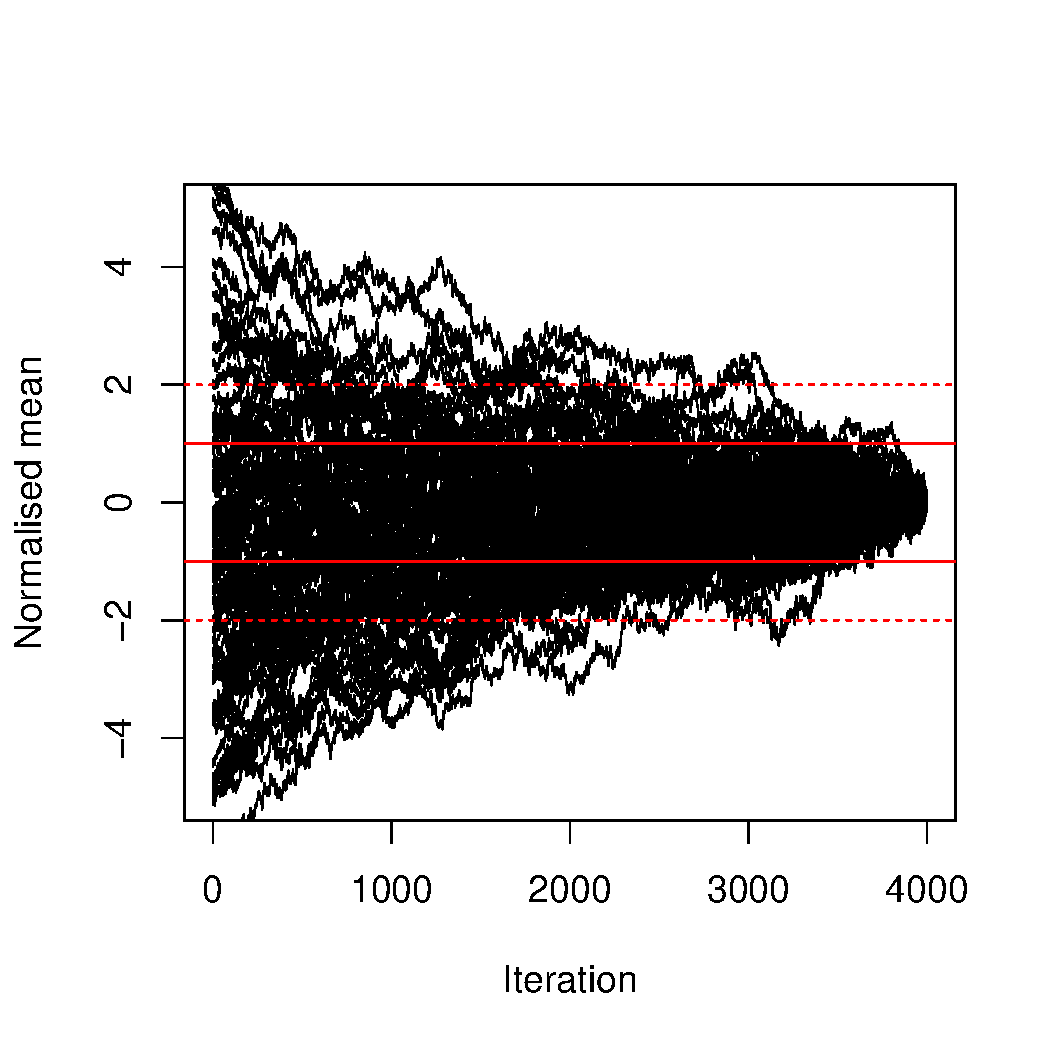
\includegraphics[width=\textwidth]{background/Figures/BHM/AllMeanParticles.pdf}
        \caption{}
        \label{}
    \end{subfigure}
    \begin{subfigure}[t]{0.45\textwidth}
    \centering
      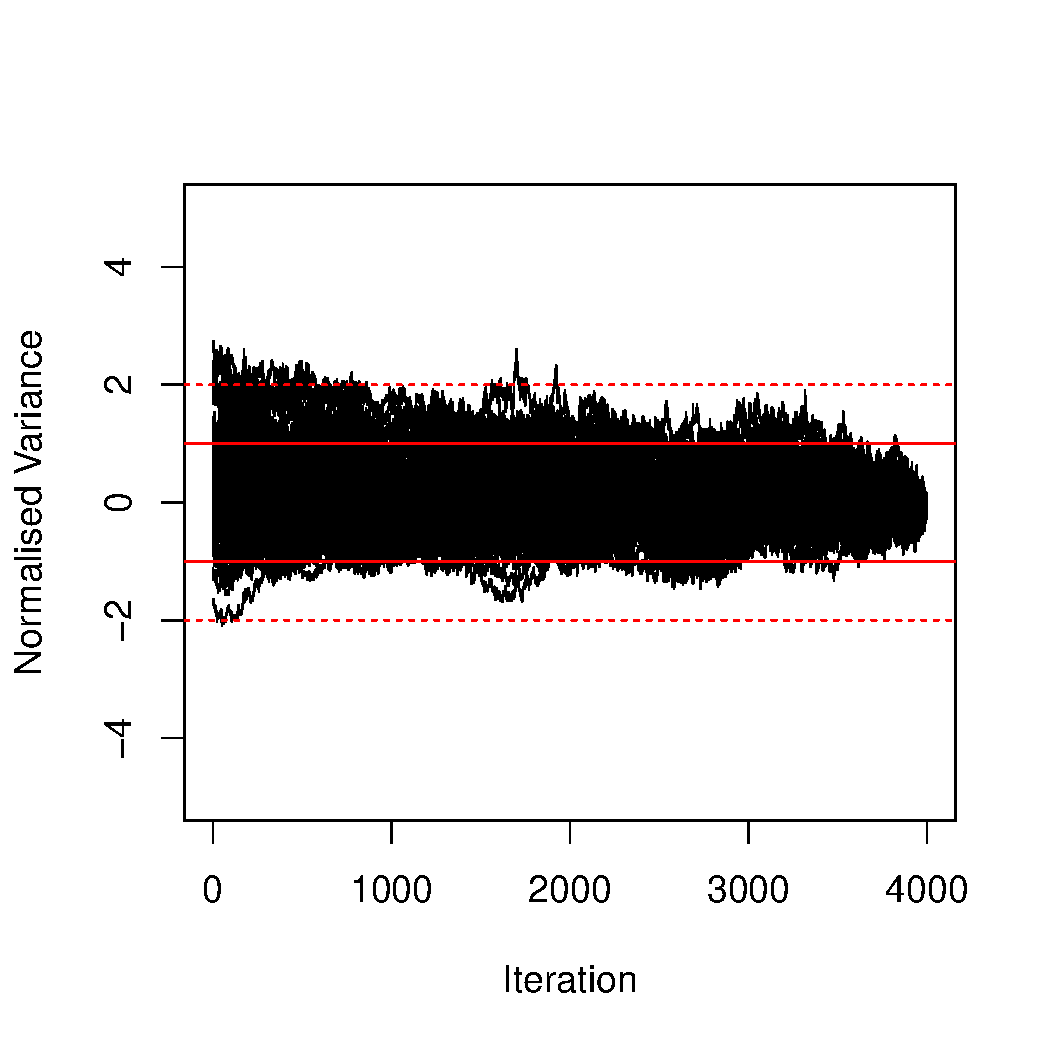
\includegraphics[width=\textwidth]{background/Figures/BHM/AllVarParticles.pdf}
        \caption{}
        \label{} 
    \end{subfigure}
\caption{Normalised mean (a) and variance (b) of each parameter in BHM model as functions of iterations. The normalisation values are the mean and variance of the ensemble of particles positions at the last iteration. Red lines show one and two sigma levels of these normalisation values. Only shown the last 4000 iterations previous to stopping the algorithm.}
\label{fig:convergence}
\end{figure}


I stop the \emph{emcee} sampling once all parameters have entered the equilibrium state and the criterium of \citet{Gong2016} \footnote{Implemented in the R package \emph{mcmcse} \citep{mcmcse}} is fulfilled. We choose this criterium because it was developed for high-dimensional problems and tested on Hierarchical Bayesian Models, as in the present work. In this criterium, the MCMC chain stops once its effective sample size (ESS) is larger than a minimum sample size. This minimum is computed using the required accuracy, $\upsilon$, for each parameter confidence interval $(1-\delta)\cdot$100\%. The ESS is the size that an independent and identically distributed sample must have to provide the desired accuracy on the parametric inference. 

The \emph{emcee} run stops once the ESS of the ensemble of walkers is greater than the minimum sample size needed for the required accuracy $\epsilon = 0.05$ on the 68\% confidence interval ($\delta = 0.32$) of each parameter.


\section{Codes}
\label{sect:code}
This Section sets out the details about the code I developed to perform the computation described throughout this chapter. First, I give a brief chronological description of the model development. Later, I will describe the details on the implementation of the charged PSO, the modified \emph{emcee}, and the GMM used to describe the field population. Finally, I will end this Section detailing the hybrid high performance computing (Hybrid-HPC) code developed to minimise the computing time of the posterior distribution in the BHM.

The first version of the Bayesian Hierarchical Model was implemented by \'Angel Berihuete in the package \emph{Stan} \citep{Stan}. It comprised a Bayesian model of the ML model of \citet{Sarro2014}. The proper motions were modelled using a single mixture of gaussians. The photometry was modelled with a Chebyshev polynomial parametrised by the length along the sequence. This length was found using a principal curve analysis and lacked physical interpretation.

I took this version and modified it in the following aspects. I included the photometric and proper motions EMB sequence, the uncertainties both in proper motion and in the photometry, and the width of the sequence modelled as the multivariate gaussian. Then, we realised that the principal curve analysis is not compatible with the deconvolution methodology. \textbf{The principal curve analysis finds the dominant curve in the observed data, and not the \emph{true} underlying relation that generates the observed data once the individual noise process for each object is accounted for. For this reason, the principal curve analysis is affected by individual uncertainties \cite[see][for the negative impact of heteroscedastic data on the related principal component analysis]{Hong2016}. Instead, we decided to model the intrinsic \emph{true} underlying photometric relation with polynomials. We use as parameter for these polynomials the \emph{true} colour $CI$, which is a more interpretable parameter than the distance along the principal curve, which was used in the previous version. Since we have one \emph{true} $CI$ for each object, the number of parameters is equal to the number of objects. We marginalised all these nuisance parameters with the aid of a prior. For this prior we introduced a probability distribution modelled by a GMM.}

Previous to the introduction of the marginalisation of the nuisance parameters, the model worked fine on samples of a few hundreds of stars. Once the marginalisation was introduced, the computing time of the model increased dramatically, rendering its application to higher data sizes impractical. At this point we decided to port the existing \emph{Stan} code into \emph
{Python}\footnote{https://www.python.org} so that we could work with the parallel \emph{emcee} code. \emph{emcee} proved to be of great use. Due to its parallelisation capabilities we were able to increase the data size from 2000 to 10,000 objects. Since the computing of the likelihood was the highest computational challenge, I developed my own routines to perform it in parallel. However, \emph{CosmoHammer} \citep{Akeret2013} turned out to be more efficient in distributing the parallel loads. I ported the BHM code into \emph{CosmoHammer} and modified the latter. The modifications ranged from data files and log entries to the introduction of priors and the handling of a Hybrid-HPC scheme using both MPI and multithreading. Despite the Hybrid-HPC scheme, the computing of the likelihood of a data set with $10^5$ objects seemed unreachable. At this point, I performed two tasks: the first was to strip the code of all auxiliary libraries calls, and the second was the vectorisation of the majority of the operations. Since the parameters of the field were held fixed, the field likelihood was computed externally for each object. The code was then fed with the data set, the field likelihood, and all the auxiliary computations reduced to a minimum. Among the reduced computation there are, for example, the Cholesky decompositions and matrix inversions of the covariance matrices of the uncertainty. Instead of doing these computation inside the code, the code was fed with the precomputed values. This further reduced the computing time.

Introducing PSO and later the charged PSO further reduced the computing time.  At this point the code was able to run on a data set with $10^5$ objects. However, convergence of the MCMC still required several weeks of computations. Once the approximation to the marginalisation integral (Eqs. \ref{eq:clmarginalps} and \ref{eq:clmarginalpb}) was introduced, the computing time reduced far more. Finally, the tuning of the \emph{emcee} parameters allowed us to increase the acceptance fraction, and reach convergence within four weeks of full computing time with an 80 cores computer cluster. It is indeed a very long time. However it is reasonable compared with our original estimates of approximately 2 years of computing time\footnote{Today, the DANCe team is working on a GPU version of the code which computes the same amount of calculations in a couple of days.}.

\subsection{The modified charged PSO}
\label{sect:chargedPSO}
As explained before, the charged PSO of \citet{Blackwell2002} was inappropriate to our objective. The metric of the parametric space of our problem is not isotropic because parameters have different length scales. For example, while fractions are constrained in the $[0,1]$ interval, proper motions parameters are allowed in the range of proper motion measurements $[-99,99]\,\mathrm{mas\cdot yr^{-1}}$. Therefore, the use of an isotropic metric results in a solution which is crowded in some parameters while is over-dispersed in others. 
To solve this issue, I modified the charged PSO by measuring distance between particles and applying the electrostatic force independently on each parameter. In such a way, the electrostatic force plays a role only when the relative distance between particles in any given parameter is smaller than $10^{-10}$. I found this value heuristically.

In the original version of  \citet{Blackwell2002}, each particle is subject to the acceleration,
\begin{equation}
\label{eq:PSOacc}
\mathbf{a}=\sum_{i\neq j} \frac{q_i \cdot q_j }{r_{ij}^3} \cdot \mathbf{r}_{ij}, \ \ \ \ p_{core} < r_{ij} < p
\end{equation}
where $q_i$ and $q_j$ are the charges of particles $i$ and $j$, and $r_{ij}$ is the distance between them. The distances $p_{core}$ and $p$ indicate the minimum and maximum distances at which the electrostatic force comes into action. Outside this range, the electrostatic force is zero. In this equation, $\mathbf{r}_{ij}= \mathbf{x}_i -\mathbf{x}_j$, where $\mathbf{x}_i,\mathbf{x}_j$ are the positions of particles $i$ and $j$. Also, $\mathbf{r}_{ij},\mathbf{x}_i,\mathbf{x}_j \subset \mathbb{R}^d$, with $d$ the dimension of the space. 

In the modified version, the distance is measured independently in each dimension of the parametric space. Thus, $\mathbf{r}_{ij}= \{x_{1,i} -x_{1,j},x_{2,i} -x_{2,j},...,x_{d,i} -x_{d,j}\}$. Also the acceleration has the form,
\begin{equation}
\label{eq:PSOacc}
\mathbf{a}=\sum_{i\neq j} \frac{q_i \cdot q_j }{r_{ij}^2} \cdot \mathbf{r}_{ij}, \ \ \ \  10^{-50} < \frac{r_{ij}}{r_{eq}} < \epsilon
\end{equation}
and it is now applied over each dimension of the parametric space. The distance $r_{eq}$ is that at which the velocity caused by the acceleration equals the mean velocity caused by the common PSO. $\epsilon$ is a free parameter which, as said previously, was set heuristically to $10^{-10}$.

\subsection{Improvements of emcee}
The modification I introduced in \emph{emcee}, although very simple, improved the acceptance fraction and mixing of the particles.
To allow the parallelisation, \citet{Foreman2013} divide the ensemble of particles in two ensembles. In the original version, the particles in one ensemble use one and the same particle in the complementary ensemble to compute their positions according to Eq. \ref{eq:stretchmove}. In the modified version, particles from one ensemble update their positions using a particle from the complementary ensemble. However, this particle is chosen randomly at each iteration. 

In a private communication with David Foreman, the developer of \emph{emcee}, he mentions that a similar modification was already introduced in a beta version of the \emph{emcee} code.

%Figure \ref{fig:emceeDANCe} compares the mixing and acceptance fractions of the original and modified versions of \emph{emcee}.
%\begin{figure}[htbp]
%\begin{center}
%%\includegraphics[width=\textwidth]{}
%\caption{Comparison between the log posterior evaluations of the original emcee version (left) and the modified one (right). }
%\label{fig:emceeDANCe}
%\end{center}
%\end{figure}
\subsection{GMM for the field population}
As mentioned earlier in this Chapter, the field population is modelled by means of two independent photometric and proper motion distributions. The MLE of the parameters of these distributions were found using the EM algorithm.  The conventional EM algorithm for GMM \citep{Dempster1977} for a mixture of $M$ gaussians goes as follows. Given a set of parameters $\theta=\{w_i,\boldsymbol{\mu}_i,\boldsymbol{\Sigma}_i\}_{i=1}^M$, were $w_i$,$\boldsymbol{\mu}_i$, and $\boldsymbol{\Sigma}_i$ are the fraction, mean and covariance matrix of gaussian component $i$, the likelihood of the data is,

\begin{equation}
p(\{\mathbf{y}_n\}_{n=1}^N|\theta)=\prod_{n=1}^N {\sum_{i=1} ^M {w_i\cdot \mathcal{N}(\mathbf{y}_n|\boldsymbol{\mu}_i,\boldsymbol{\Sigma}_i)}}.
\end{equation}

To solve the problem, the EM algorithm requires  a set of $N$ variables, $\{\boldsymbol{z}_n\}_{n=1}^N$, of dimension $M$. The variable $z_{n,i}$ represent the probability that observation $y_n$ was drawn from gaussian $i$. Therefore,

\begin{equation}
1=\sum_{i=1}^M z_{n,i}.
\end{equation}

These $\boldsymbol{z}$ latent variables are found as
\begin{equation}
z_{n,i}= \frac{w_i\cdot \mathcal{N}(\mathbf{y}_n|\boldsymbol{\mu}_i,\boldsymbol{\Sigma}_i)}{\sum_{i=1}^M w_i\cdot \mathcal{N}(\mathbf{y}_n|\boldsymbol{\mu}_i,\boldsymbol{\Sigma}_i)}.
\end{equation}

The EM works, as its name indicates, by maximising the expected value of the likelihood. The latter is given by
\begin{equation}
E[p(\{\mathbf{y}_n\}_{n=1}^N|\theta)]=\prod_{n=1}^N {\sum_{i=1} ^M {z_{n,i}\cdot w_i\cdot \mathcal{N}(\mathbf{y}_n|\boldsymbol{\mu}_i,\boldsymbol{\Sigma}_i)}}.
\end{equation}

The previous expectation is maximal when,
\begin{align}
w_i &= \frac{1}{N} \sum_{n=1}^N z_{n,i}, \\
\boldsymbol{\mu}_i &= \frac{1}{\sum_{n=1}^N z_{n,i}} \sum_{n=1}^N z_{n,i}\cdot \mathbf{y}_n,\\
\boldsymbol{\Sigma}_i &= \frac{1}{\sum_{n=1}^N z_{n,i}} \sum_{n=1}^N z_{n,i}\cdot (\mathbf{y}_n - \boldsymbol{\mu}_i)\times(\mathbf{y}_n-\boldsymbol{\mu}_i)^T.
\end{align}

The modified version of the GMM, which includes a uniform distribution, is now a particular case of the GMM. This can be viewed as a gaussian distribution with fixed parameters and a constant probability $c$ given by the uniform distribution. The new expectation is then,
\begin{equation}
E[p(\{\mathbf{y}_n\}_{n=1}^N|\theta)]=\prod_{n=1}^N {\left[z_{n,0}\cdot w_0 \cdot c + \sum_{i=1} ^M {z_{n,i}\cdot w_i\cdot \mathcal{N}(\mathbf{y}_n|\boldsymbol{\mu}_i,\boldsymbol{\Sigma}_i)}\right]}.
\end{equation}

The maximisation step remains identical except for the indices. There are now $M+1$ fractions $w_i$, with $i=0,1,...,M$, and the means and covariances run from $i=1,...,M$.

Regarding the photometric GMM of the field, and given that the photometry has missing values, we use the EM algorithm of \citet{McMichael1996}. This algorithm was developed to obtain the MLE of data sets containing objects with missing values. A more recent version has been developed by \citet{Lin2006}, however, this assumes that the missing entries are randomly distributed (missing at random). However,  as mentioned earlier, the missing values in the photometry of the DANCE DR2 are not randomly distributed.

In the algorithm of \citet{McMichael1996}, there is a set of $N$ gain matrices, one for each datum. Each $M_n$ matrix is an identity matrix in which the rows of the corresponding missing value have been deleted. Thus, the expected value of the likelihood is now,

\begin{equation}
E[p(\{\mathbf{y}_n\}_{n=1}^N|\theta)]=\prod_{n=1}^N {\sum_{i=1} ^M {z_{n,i}\cdot w_i\cdot \mathcal{N}(\mathbf{y}_n|M_n \boldsymbol{\mu}_i,M_n\boldsymbol{\Sigma}_i M_n)}}.
\end{equation}

The maximisation step is now,

\begin{align}
w_i &= \frac{1}{N} \sum_{n=1}^N z_{n,i}, \\
\boldsymbol{\mu}_i &= \frac{ \sum_{n=1}^N z_{n,i}\cdot H_n \mathbf{y}_n}{\sum_{n=1}^N z_{n,i} H_n M_n}
\end{align}
with 
\begin{equation}
H_i=M_i^T(M\Sigma_i M^T)^{-1}
\end{equation}

The maximisation step has no analytical solution for the covariance matrix. Therefore, a modified steepest descent is used

\begin{equation}
\Sigma_i \leftarrow \Sigma_i + \frac{\rho}{2}\cdot \Sigma_i\Delta_i\Sigma_i,
\end{equation}
with $\Delta_i$ given by

\begin{equation}
\Delta_i=  \frac{1}{\sum_{n=1}^N z_{n,i}}\cdot \sum_{n=1}^N z_{n,i} \cdot \left[H_n(\mathbf{y}_n -  M_n \boldsymbol{\mu}_i) \times  (\mathbf{y}_n -  M_n \boldsymbol{\mu}_i)^TH_n^T - H_nI\right].
\end{equation}
 
 This algorithm preserves the monotonic convergence of the conventional EM, and returns positive definite matrices provided that $\rho < 2$. For details and validation of this algorithm see \citet{McMichael1996}.

\subsection{Hybrid-HPC implementations}
\label{sect:HHPC}
As I outlined before, the parallel computing approach was an unavoidable step. Once the code was ported to \emph{Python} and \emph{CosmoHammer}, I modified the latter to better fit our needs. The modifications were mainly on the management of input and output files and the python \emph{multiprocessing} package for the multithreaded computing of likelihoods. Also, I striped some of its original functions to reduce memory usage and implemented some others, like the use of initial positions for the particles.

In the Hybrid-HPC approach, the particles of \emph{emcee} are distributed on the nodes of the computing cluster by means of the MPI protocol. Then, each core in the node computes the likelihood of one fraction of the objects in the data set. This Hybrid-HPC code was implemented and tested in different computing cluster architectures. For the cluster at the Centre of Astrobiology (CAB, Villanueva de la ca\~nada, Madrid, Spain), I used a configuration of 6 nodes each with 12 cores. For the cluster at the University of C\'adiz, (Andalucía, Spain) I used a configuration of 5 nodes each with 16 cores.

However, the  Hybrid-HPC approach was not the best solution at the Infrastructure de Calcul Intensive et de Donées\footnote{https://gricad.univ-grenoble-alpes.fr}of the University of Grenoble Alpes. At the Froggy\footnote{https://ciment.ujf-grenoble.fr/wiki-pub/index.php/Hardware:Froggy} cluster, the code continuously render errors of communication. For this reason, I implemented a MPI-only version of the code. In this version, the multithreading approach is left aside. Instead, the totality of the available cores is fully dedicated to the computing of the likelihood. Each of the $n$ cores computes the likelihood of the $n$th fraction of the objects in the data set. Once the likelihood of all particles has been computed, the master node evaluates the new positions of the particles.

I finish this chapter with a brief description of the difficulties faced in the development and testing of the BHM code. As the code evolved in complexity, my computational skills were compelled to evolve as well. I started by learning R and solving some toy problems on it. Later, when the dimensionality of the posterior increased I learned \emph{Stan}. When the data set increased in size, we faced the parallelisation, so I learned Python and MPI. Once these versions were operable, I was forced to deal with libraries, from the common, numpy, scipy and numba, to the linking of modules and libraries. Finally, when dealing with several clusters I learned the queue languages Condor, slurm and OAR. Currently, I am working on the improvement (memory allocation and data distribution) of the GPU implementation of the BHM code.  



